\documentclass[a4paper, titlepage, 12pt]{article}
\usepackage{graphicx}
\usepackage{amsmath}
\usepackage[margin=1in]{geometry}
\usepackage{float}

\begin{document}

	\title{EE 141 Controller Design for a Fast Tool Servo}
	\author{Sidharth Bambah \\ UID: 904 787 435 \\\\
			Robert Carey \\ UID: 004 940 804}
	\date{10 March 2018}
	\maketitle
	
	\section{Introduction}
		The purpose of this project is to designe controllers for a Fast Tool
		Servo (FTS) system. The tasks of the project are as follows: \\
		\begin{enumerate}
			\item Design an OpAmp-based high-bandwidth controller for the current
			control loop to drive the actuator.
			\item Identify the dynamics of the FTS electromechanical plant from
			the measured frequency response data
			\item Design a position controller that minimizes tracking error for
			step and sinusoidal inputs at steady state in the presence of sensor
			noise.
		\end{enumerate}
		\begin{figure}
			\centering
			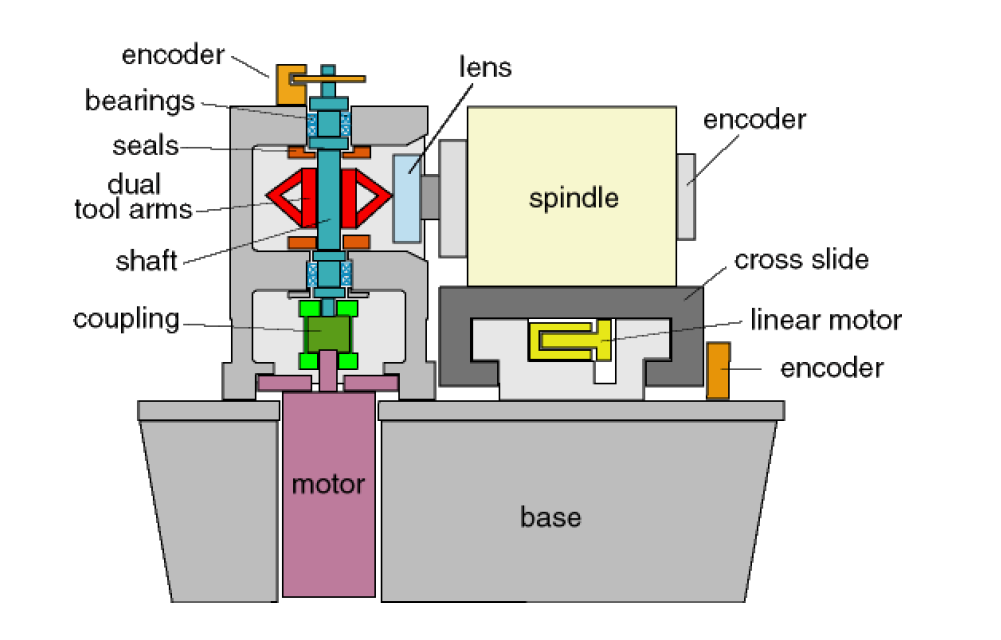
\includegraphics[width=\linewidth]{images/fts_schematics.PNG}
			\caption{FTS Schematics}
			\label{fts_schematics}
		\end{figure}
		The Fast Tool Servo schematics are given in Figure \ref{fts_schematics}. \\\\
		\begin{figure}
			\centering
			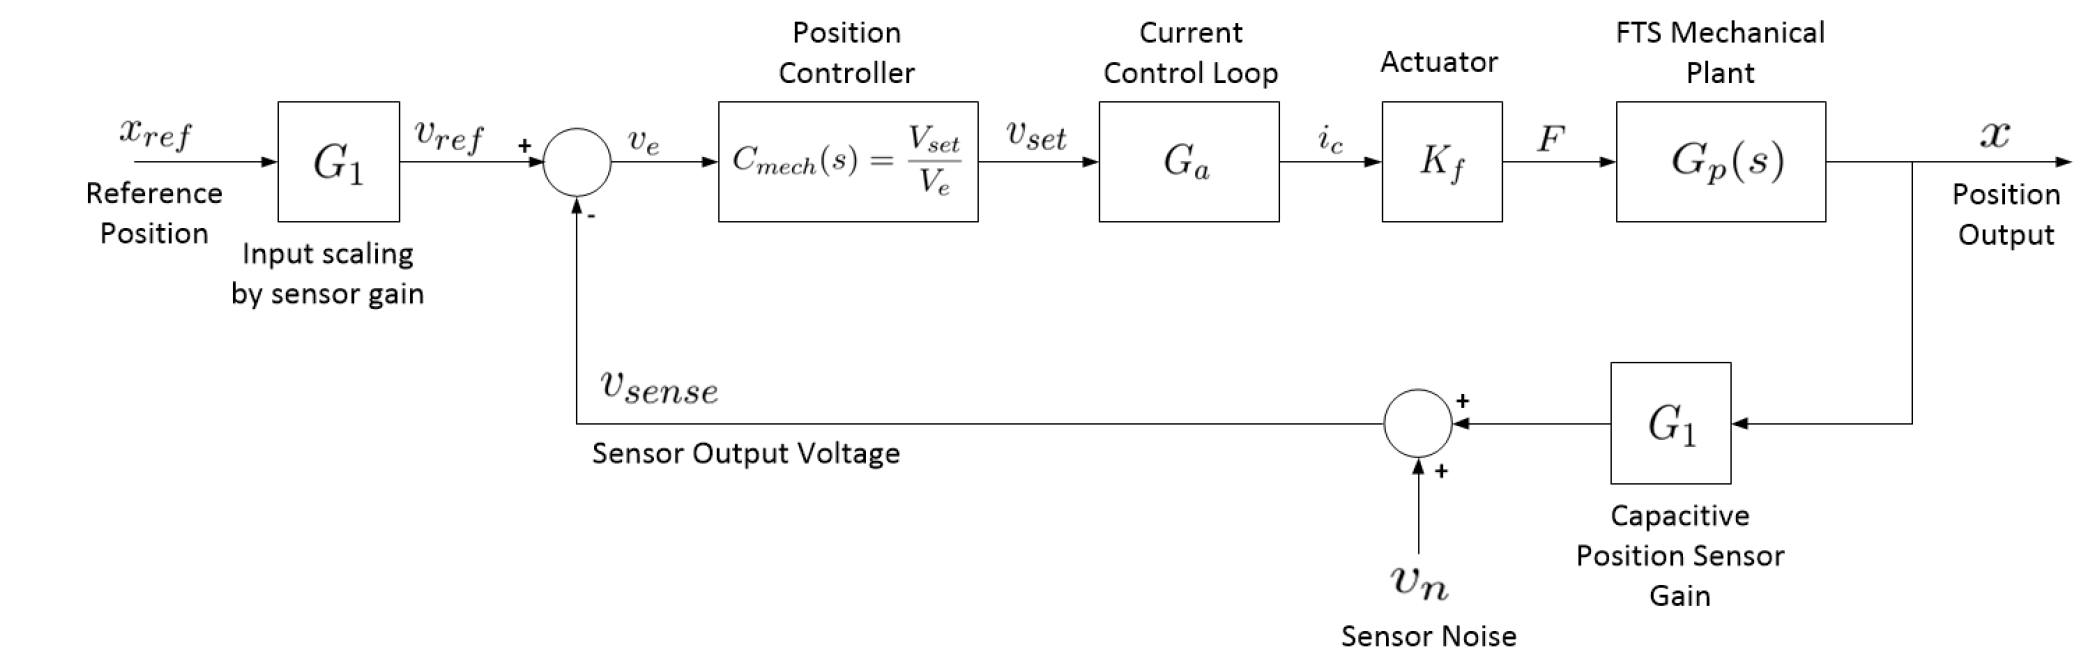
\includegraphics[width=\linewidth]{images/control_loop.PNG}
			\caption{Fast Tool Servo Overall Control Loop}
			\label{overall_control_loop}
		\end{figure}
		The overall control loop of the FTS system used in this project is given
		in Figure \ref{overall_control_loop} and shows that the ultimate goal for
		the system is to control the position of the cutting tool x(t) such that
		it tracks the position trajectory $x_{ref}(t)$. \\\\
		As can be seen in the entire control loop the system consists of the
		following parts: \\
		\begin{itemize}
		\item \textbf{FTS mechanical plant} $G_p(s)$: The actuator force results in
		the displacement of the cutting tool.
		\item \textbf{Actuator}: The motor where the current $i_c$ is regulated to
		generate the required force for the mechanical plant. Can be described
		by a fixed gain of $K_f = 20 N/A$.
		\item \textbf{Current Control Loop}: Controls the current $i_c$, which
		drives the actuator, based on the input voltage $v_{set}$. The loop is
		fast enough that the resulting dynamics are fast enough compared to the
		bandwidth that they can be ignored and the loop can be replaced with a
		constant gain $G_a=-0.5 A/V$.
		\item \textbf{Position Controller} $C_{mech}(s)$: Gets the error between
		the reference voltage $v_{ref}$ and the sensor output voltage $v_{sense}$
		and generates the voltage $v_{set}$ to drive the control loop.
		\item \textbf{Position Sensor}: A capacitive displacement sensor that
		measures the position of the cutting tool. It can be modeled by a constant
		gain $G_1 = 5*10^5V/m$ and the output is assumed to be corrupted by
		measurement noise $v_n$.
		\end{itemize}
	\section{Current Control Loop Design}
		\begin{figure}
			\centering
			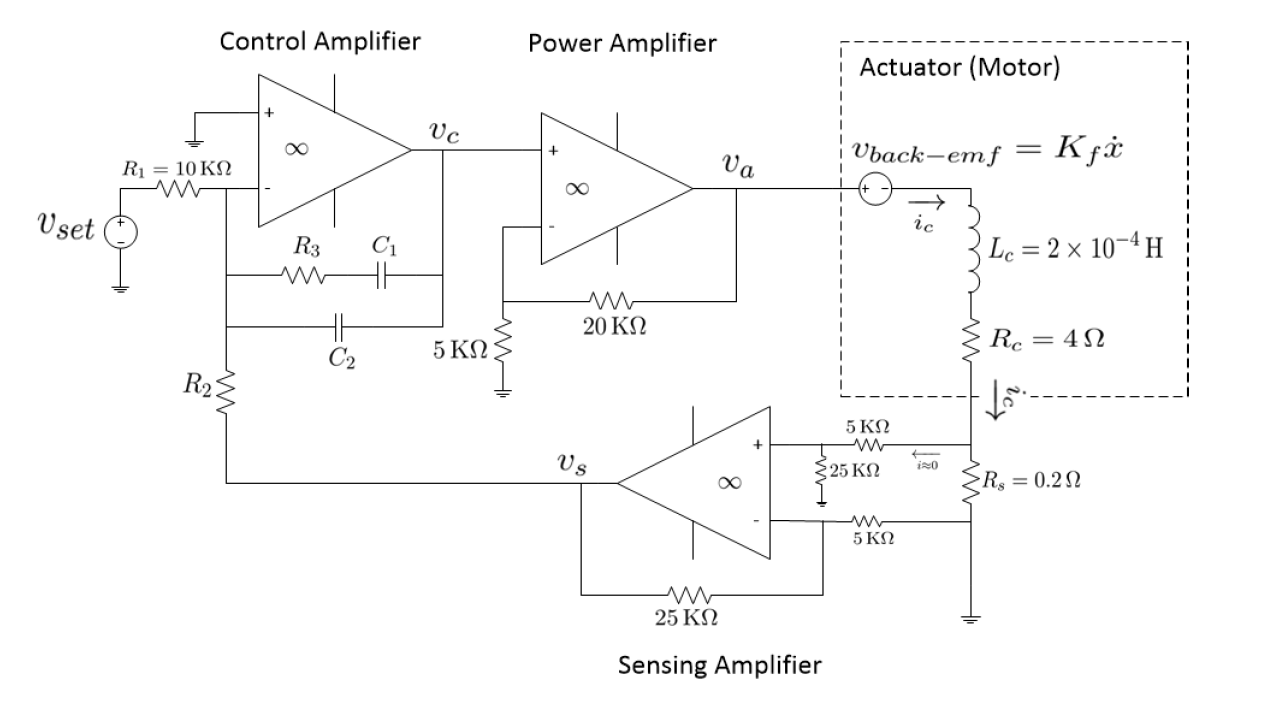
\includegraphics[width=\linewidth]{images/current_loop_schematic.PNG}
			\caption{Current Control Loop Schematic}
			\label{current_loop_schematic}
		\end{figure}
		\begin{figure}
			\centering
			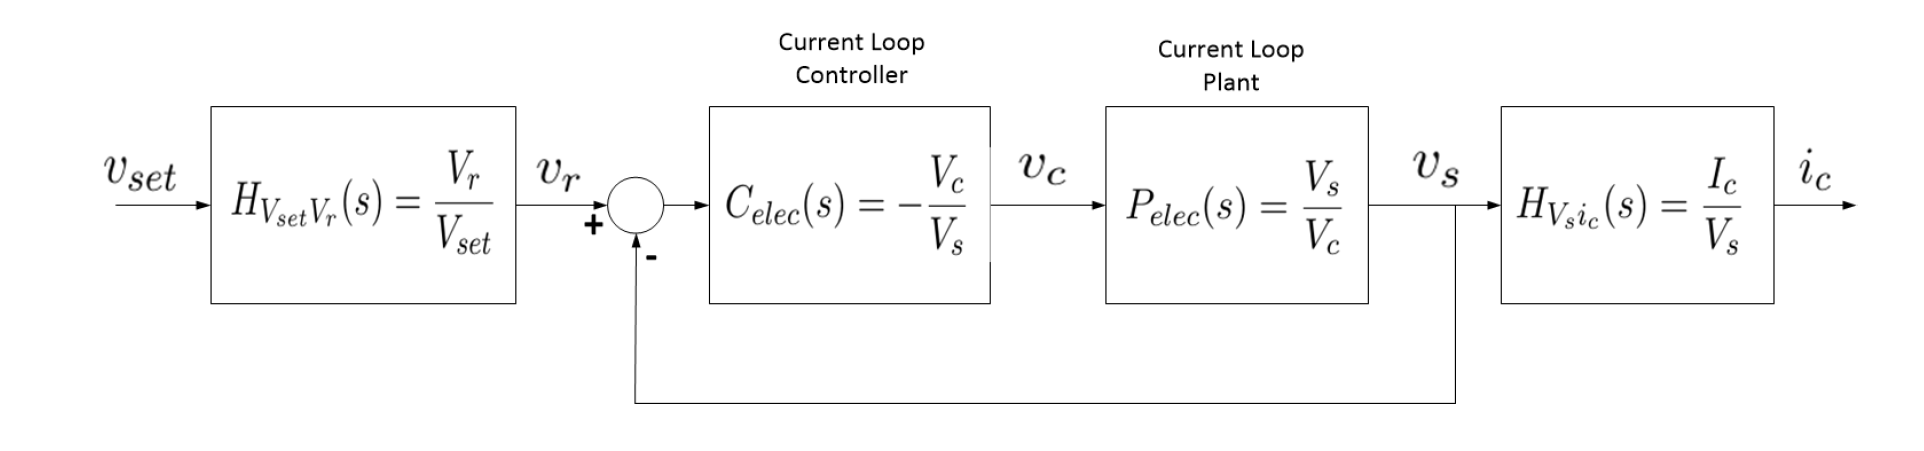
\includegraphics[width=\linewidth]{images/current_loop_block.PNG}
			\caption{Current Control Loop Block Diagram}
			\label{current_loop_block}
		\end{figure}
		The first step is to design the current loop plant and current loop
		controller. The schematic for the current control loop is given in Figure
		\ref{current_loop_schematic}. Another representation of the current
		control loop, in the form of a block diagram is given in Figure
		\ref{current_loop_block}. \\\\
		\begin{figure}
			\centering
			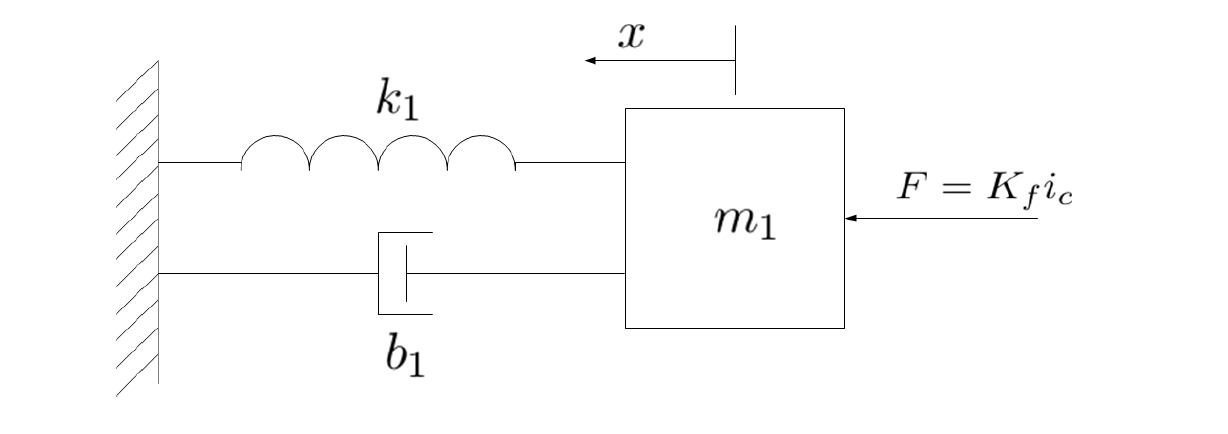
\includegraphics[width=\linewidth]{images/mechanical_model.PNG}
			\caption{Model for mechanical dynamics of FTS}
			\label{mechanical_model}
		\end{figure}
		As can be seen in the schematics, the back electromotive force (back emf)
		from the actuator can be modeled as a dependent voltage source with voltage
		proportional to the velocity of the cutting tool: $v_{back\_emf} = K_f\dot{x}(t)$.
		Additionally, the force generated by the actuator is assumed to be proportional
		to the actuator current with the same gain: $F(t) = K_fi_c(t)$. A model
		describing the mechanical dynamics of the FTS is shown in Figure
		\ref{mechanical_model} where the actuator force F(t) is applied to a mass
		$m_1$ subject to resistance by a spring $k_1$ and a damper $b_1$. \\\\
		\begin{enumerate}
			\item Identifying $P_{elec}(s) = \frac{V_s(s)}{V_c(s)}$ with Back EMF \\\\
			The derivation for $P_{elec}(s)$ with back emf included is given below.
			In this case, the FTS schematics given in Figure \ref{fts_schematics}
			are taken into account and reflected in the plant transfer function.
			\begin{figure}[H]
				\centering
				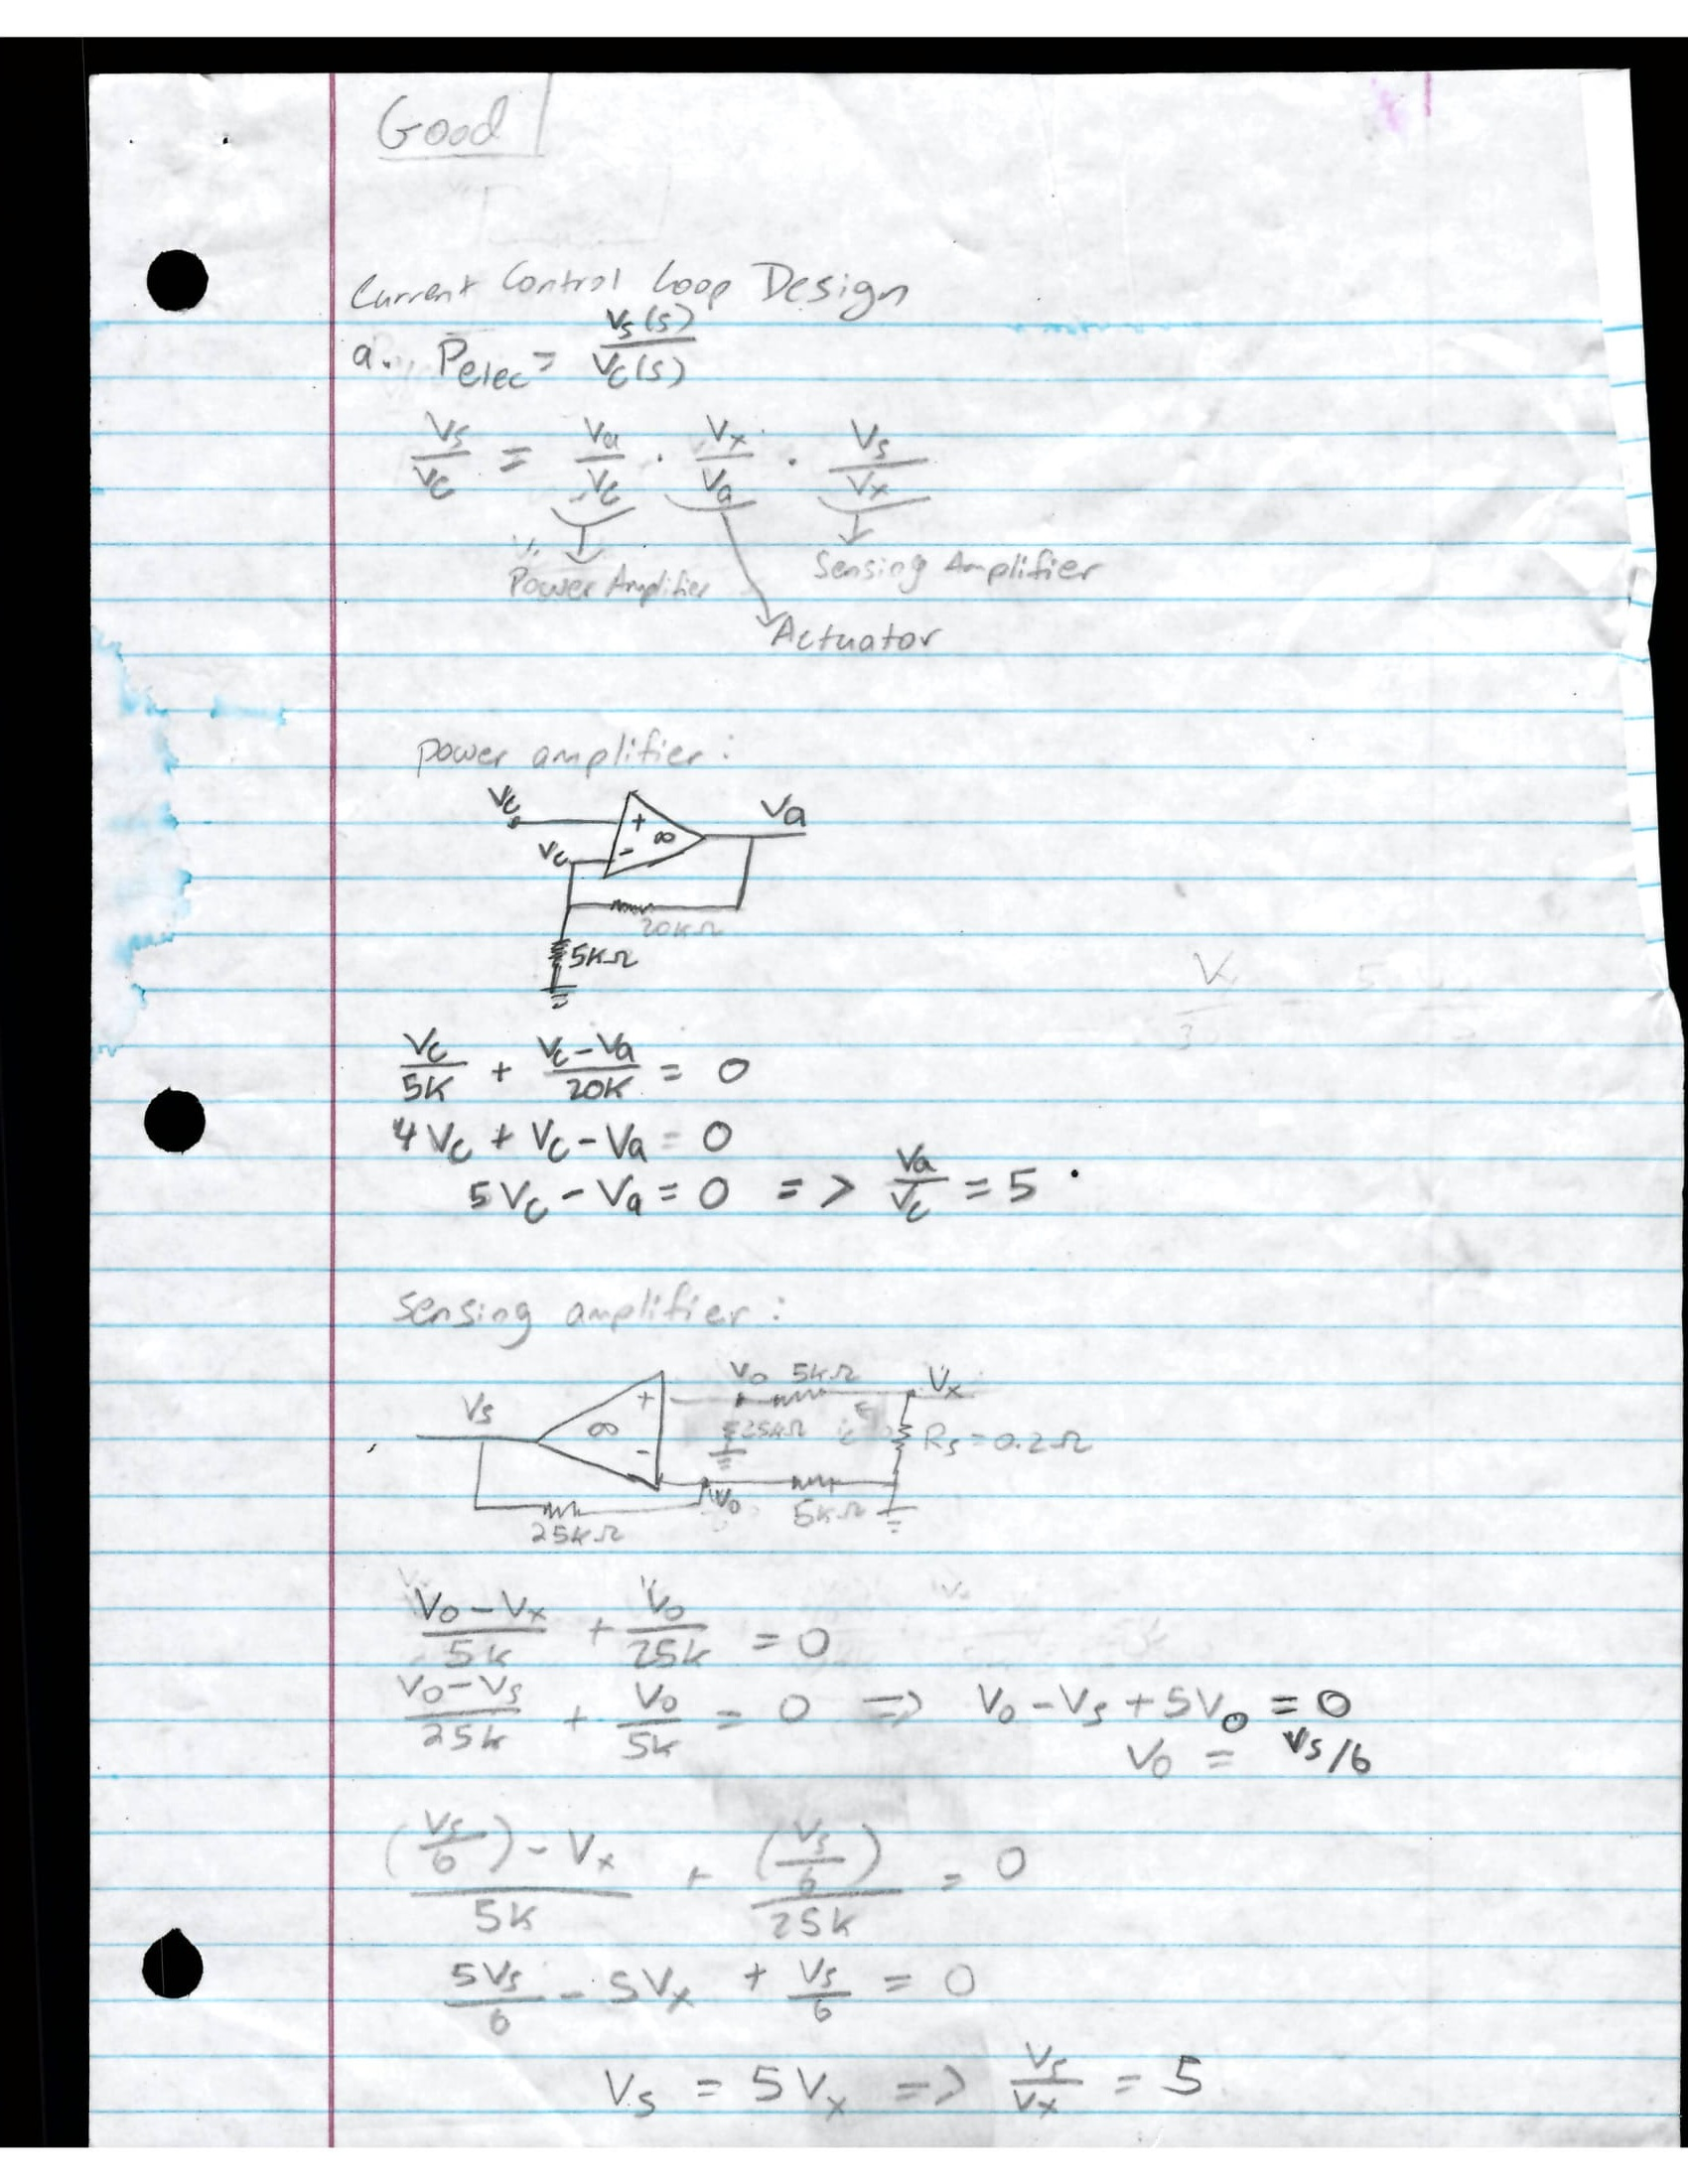
\includegraphics[width=\linewidth]{images/p_elec_emf_1.jpg}
			\end{figure}
			\begin{figure}[H]
				\centering
				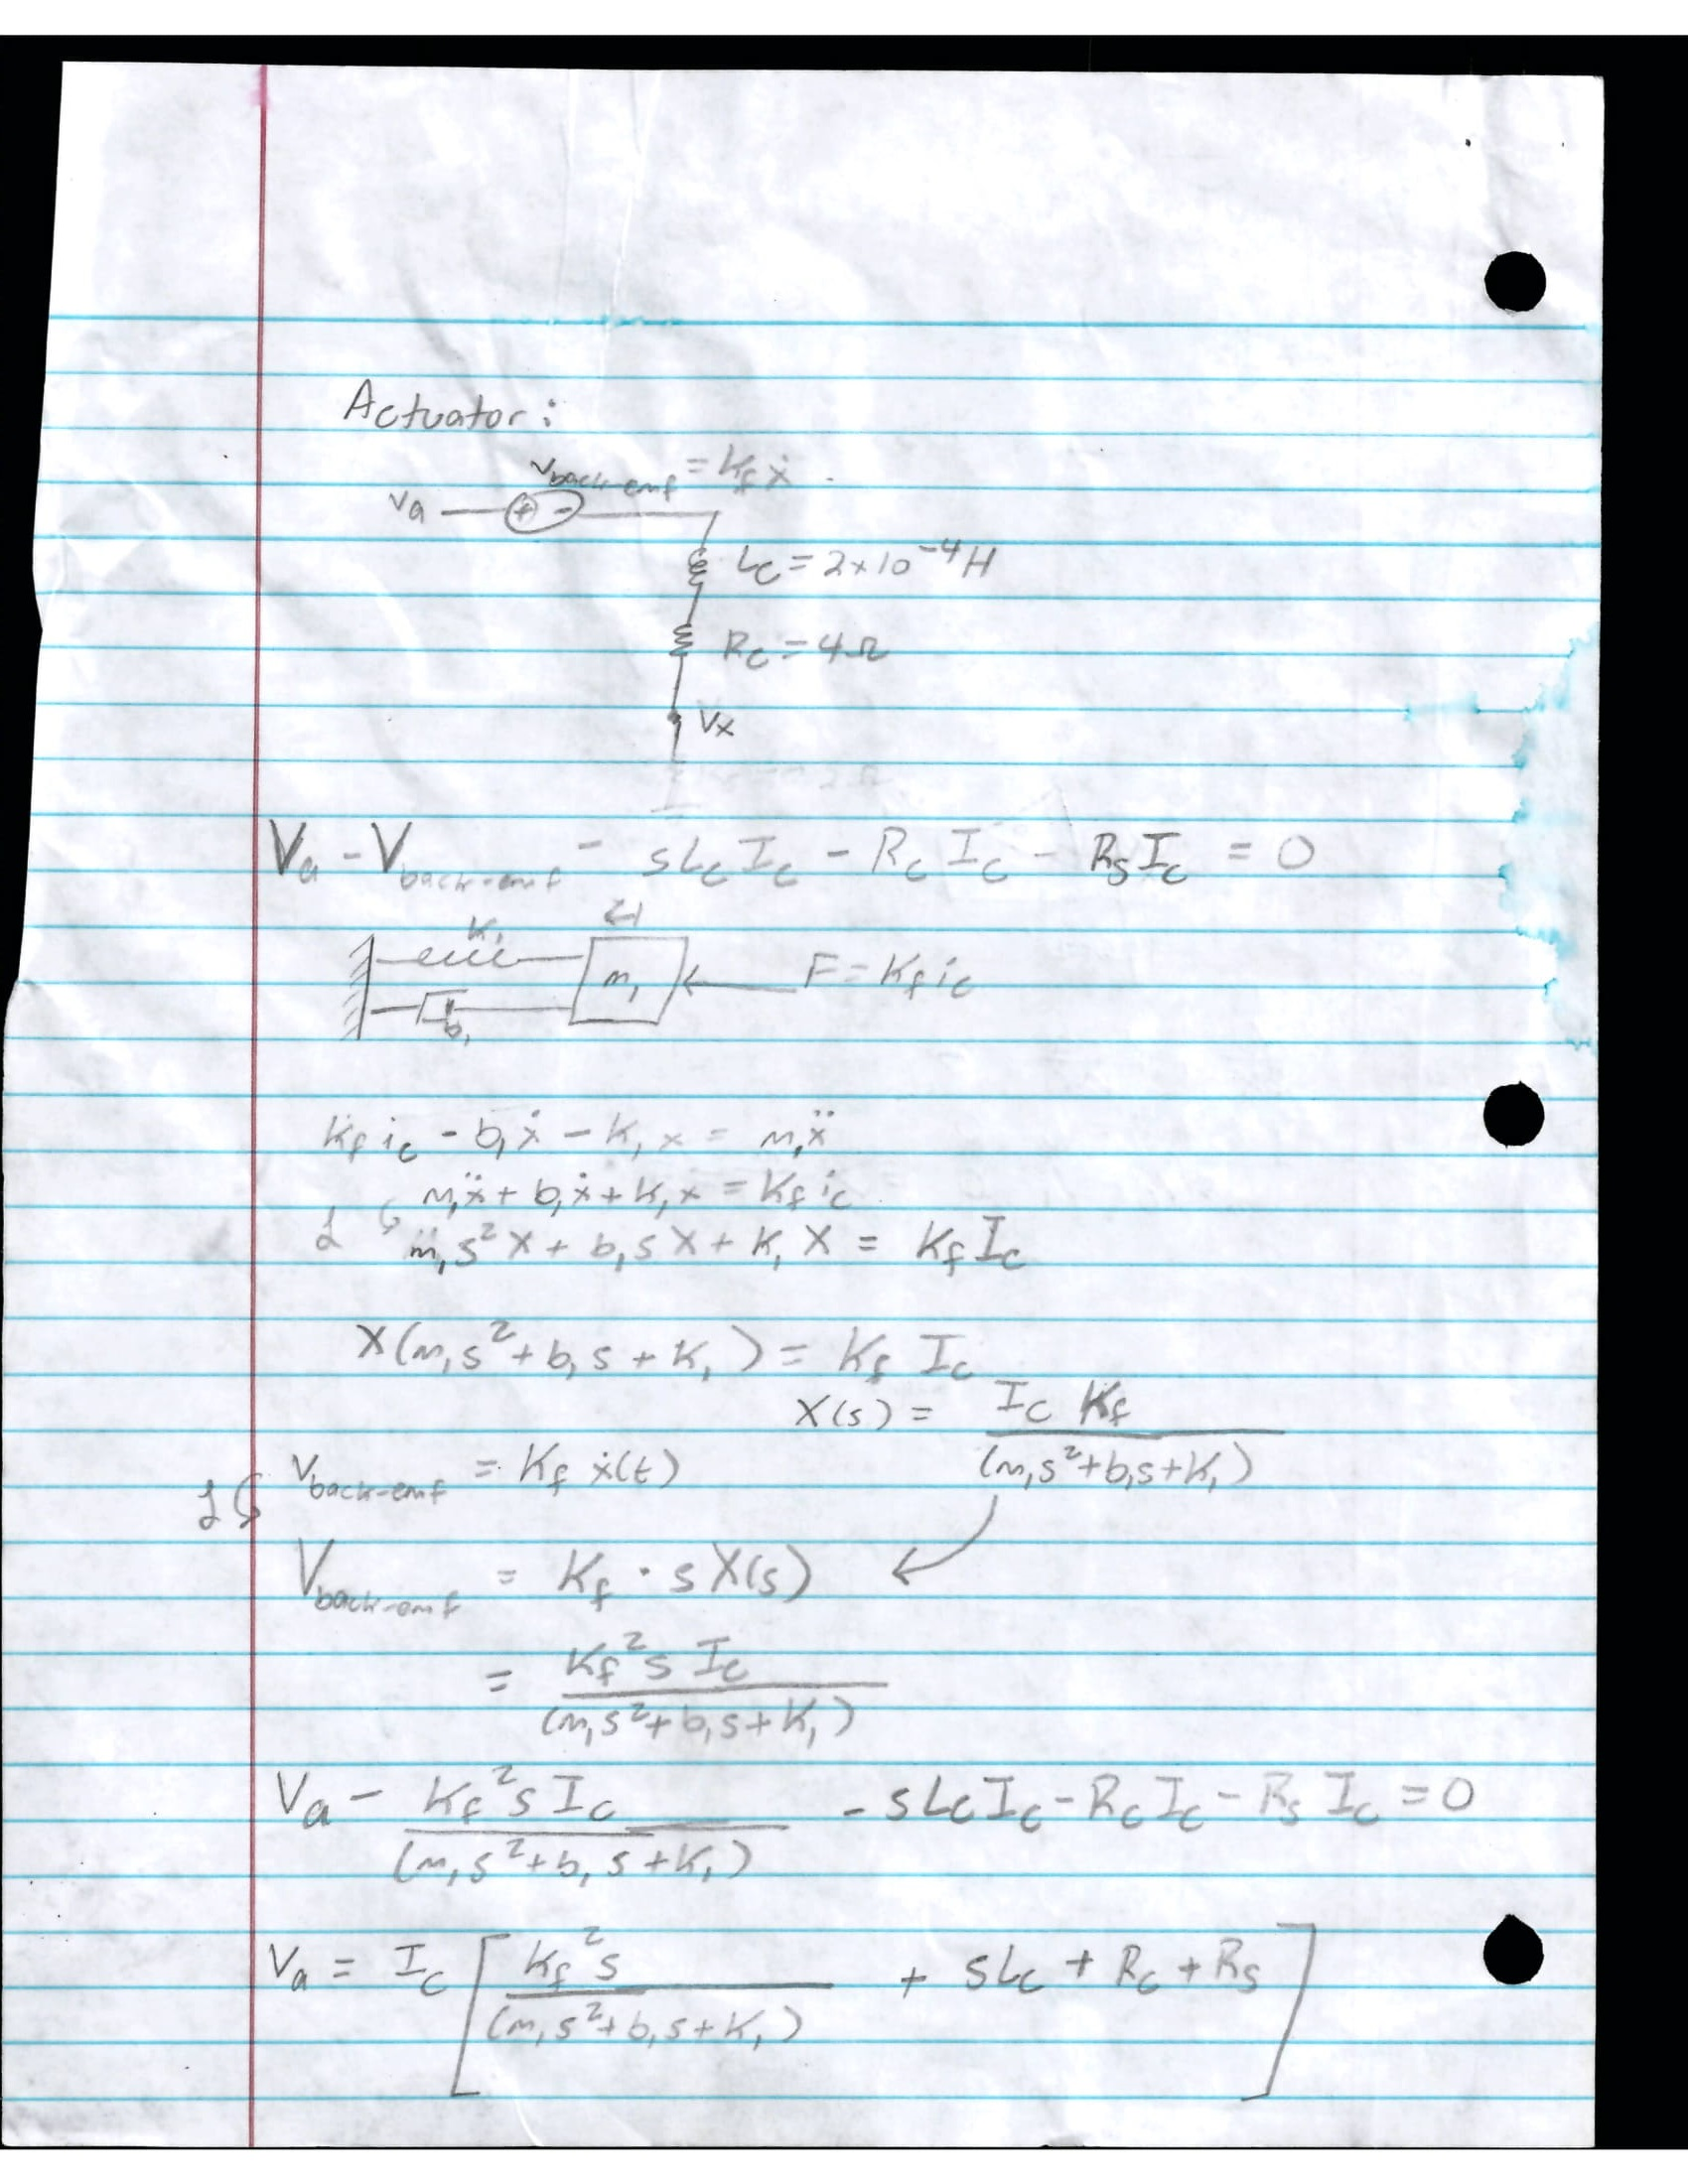
\includegraphics[width=\linewidth]{images/p_elec_emf_2.jpg}
			\end{figure}
			\begin{figure}[H]
				\centering
				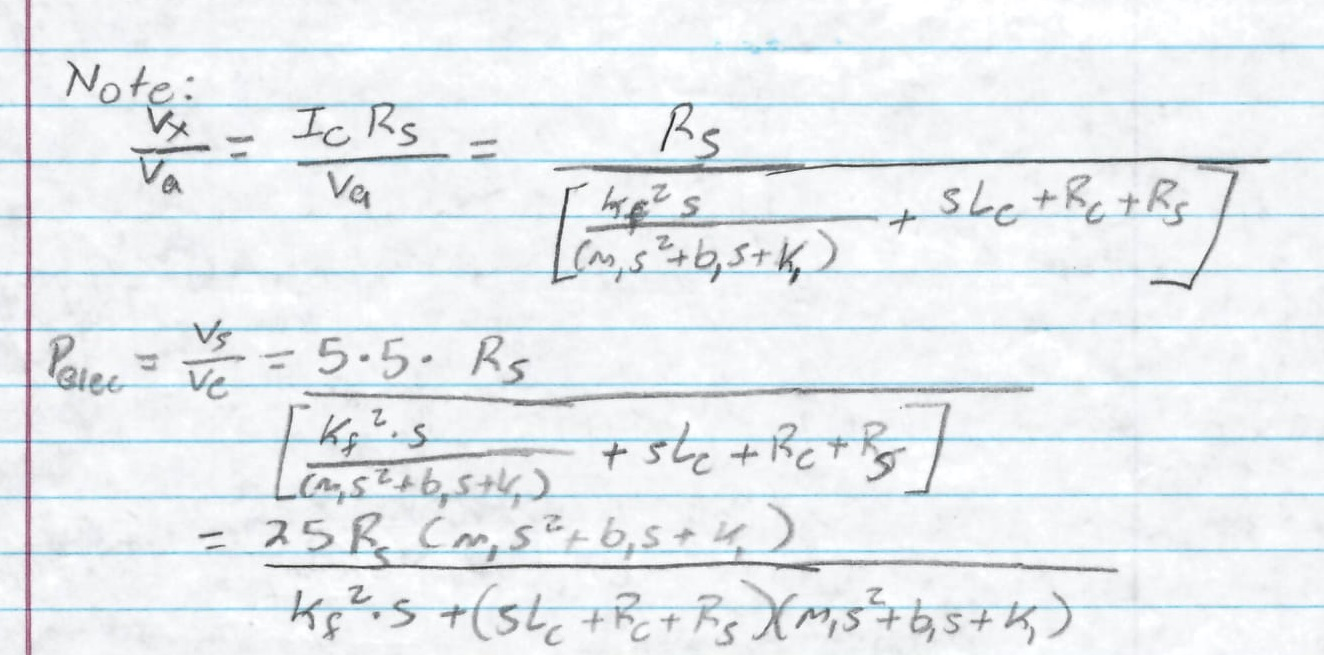
\includegraphics[width=\linewidth]{images/p_elec_emf_3.jpg}
			\end{figure}
			\item Identifying $P_{elec}(s) = \frac{V_s(s)}{V_c(s)}$ without Back EMF \\\\
			The derivation for $P_{elec}(s)$ with back emf assumed to be zero is
			given below. In this case, the FTS dynamics given in Figure \ref{fts_schematics}
			have no effect on the transfer function.
			\begin{figure}[H]
				\centering
				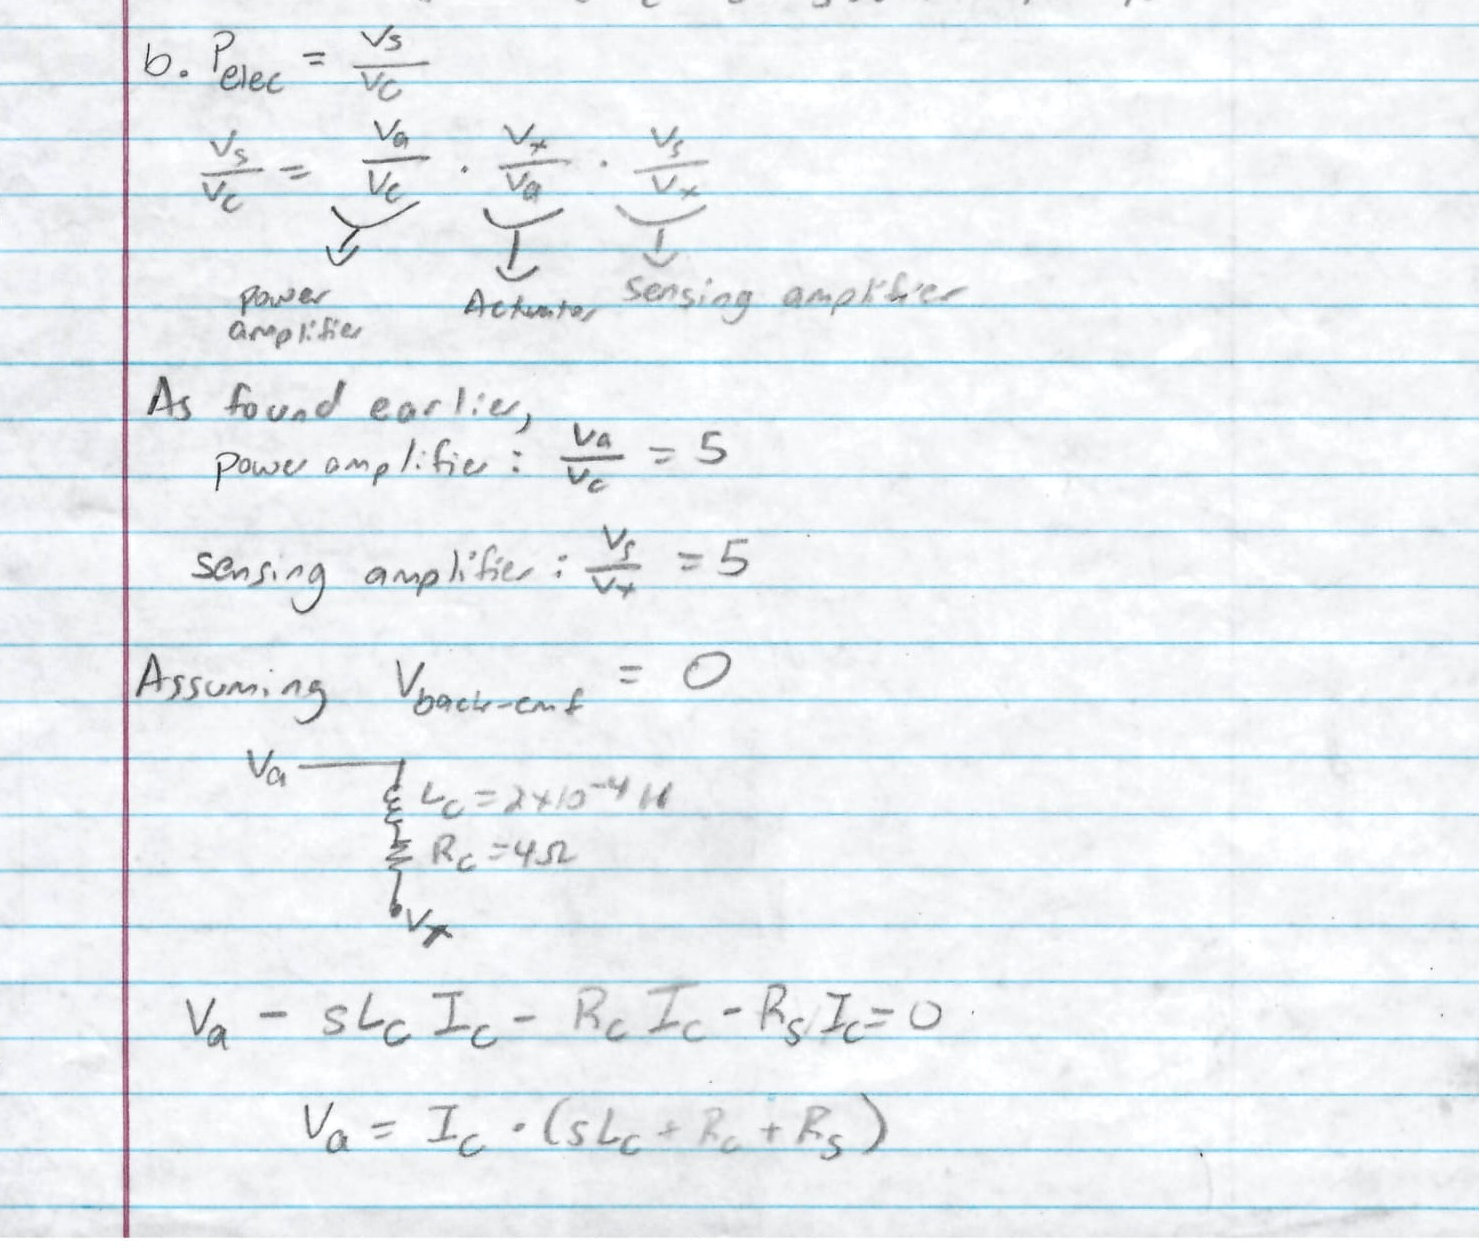
\includegraphics[width=\linewidth]{images/p_elec_noemf_1.jpg}
			\end{figure}
			\begin{figure}[H]
				\centering
				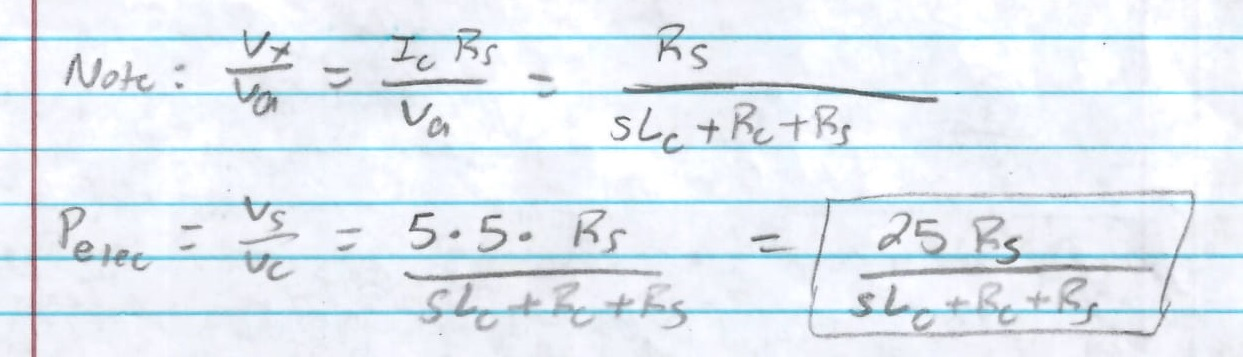
\includegraphics[width=\linewidth]{images/p_elec_noemf_2.jpg}
			\end{figure}
			\item Show that at high frequencies, both transfer functions are the same \\\\
			As can be seen in the analysis below, both versions of $P_{elec}(s)$,
			with and without back emf, are the same at high frequencies. Because
			of this fact, the back emf voltage can be assumed zero for the 
			controller design portion.
			\begin{figure}[H]
				\centering
				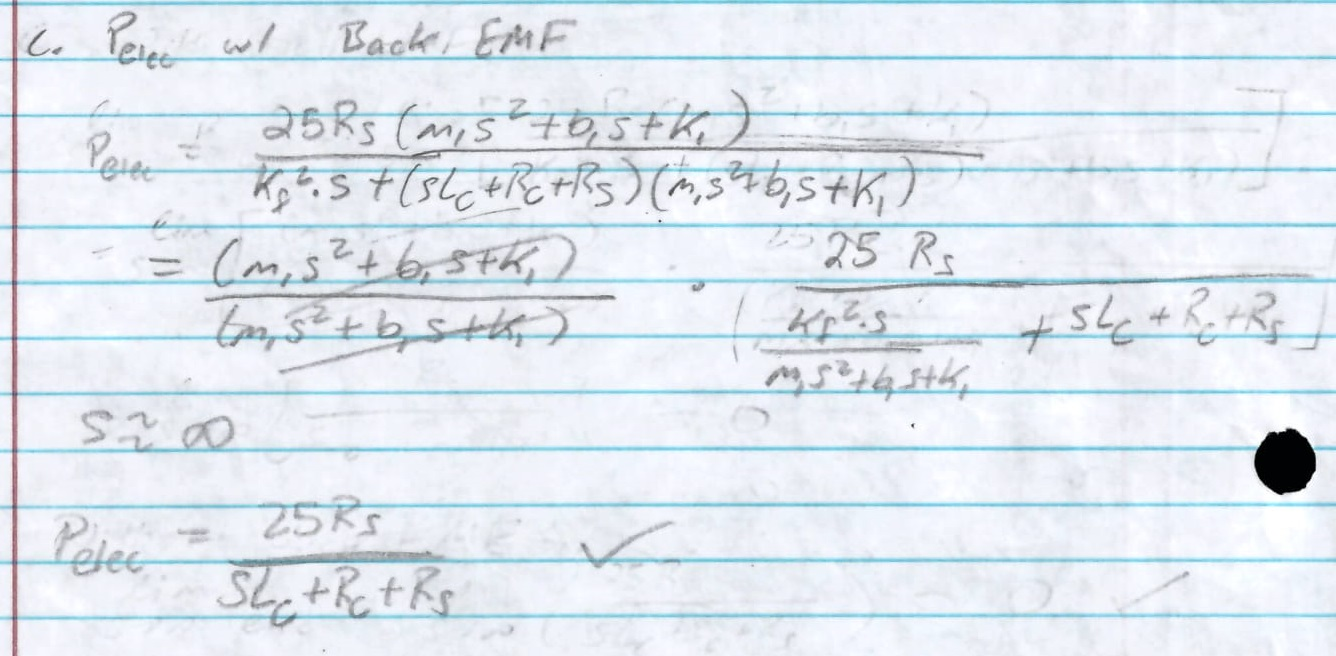
\includegraphics[width=\linewidth]{images/p_elec_high_freq.jpg}
			\end{figure}
			\item Design $C_{elec} = -\frac{V_c(s)}{V_s(s)}$ \\\\
			The derivation of the current loop controller with a gain crossover
			frequency of $\omega_c = 6*10^5 rad/sec$ and a minimum phase margin
			of $PM \geq 60\circ$ is given below. Given that the input voltage of
			$v_{set} = 0$ results in a steady-state actuator coil current of
			$i_c = 5A$, it can be found that the full closed-loop current drive has
			a gain of $G_a = -0.5 A/V$. Also, given that $R_1 = 10K\Omega$ and
			$R_s = 0.2\Omega$, we can find the resulting component values of $R_1$, 
			$R_3$, $C_1$, and $C_2$.
			\begin{figure}[H]
				\centering
				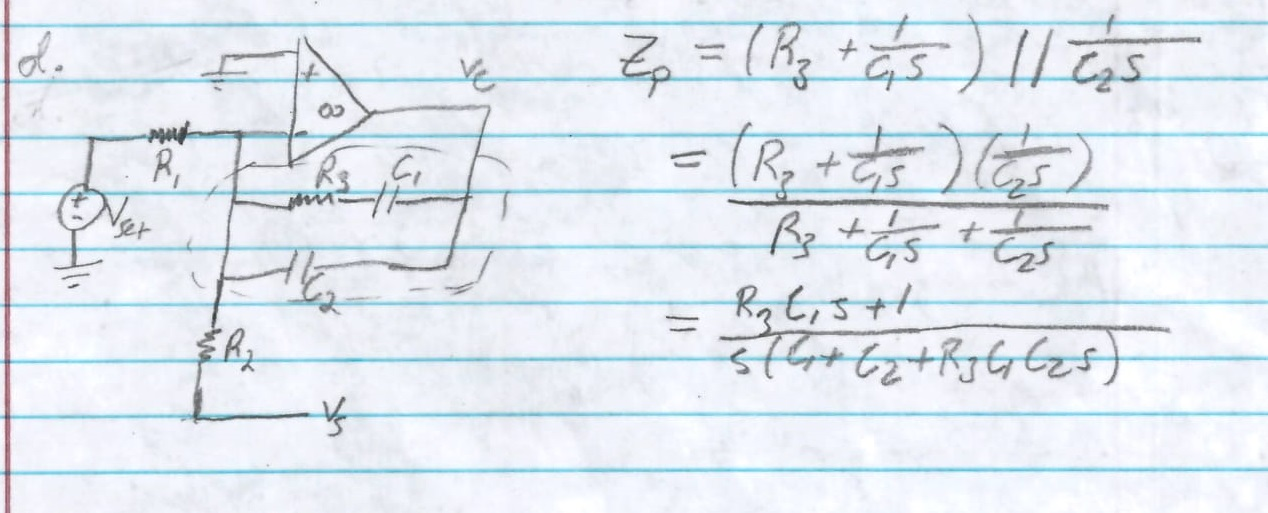
\includegraphics[width=\linewidth]{images/c_elec_1.jpg}
			\end{figure}
			\begin{figure}[H]
				\centering
				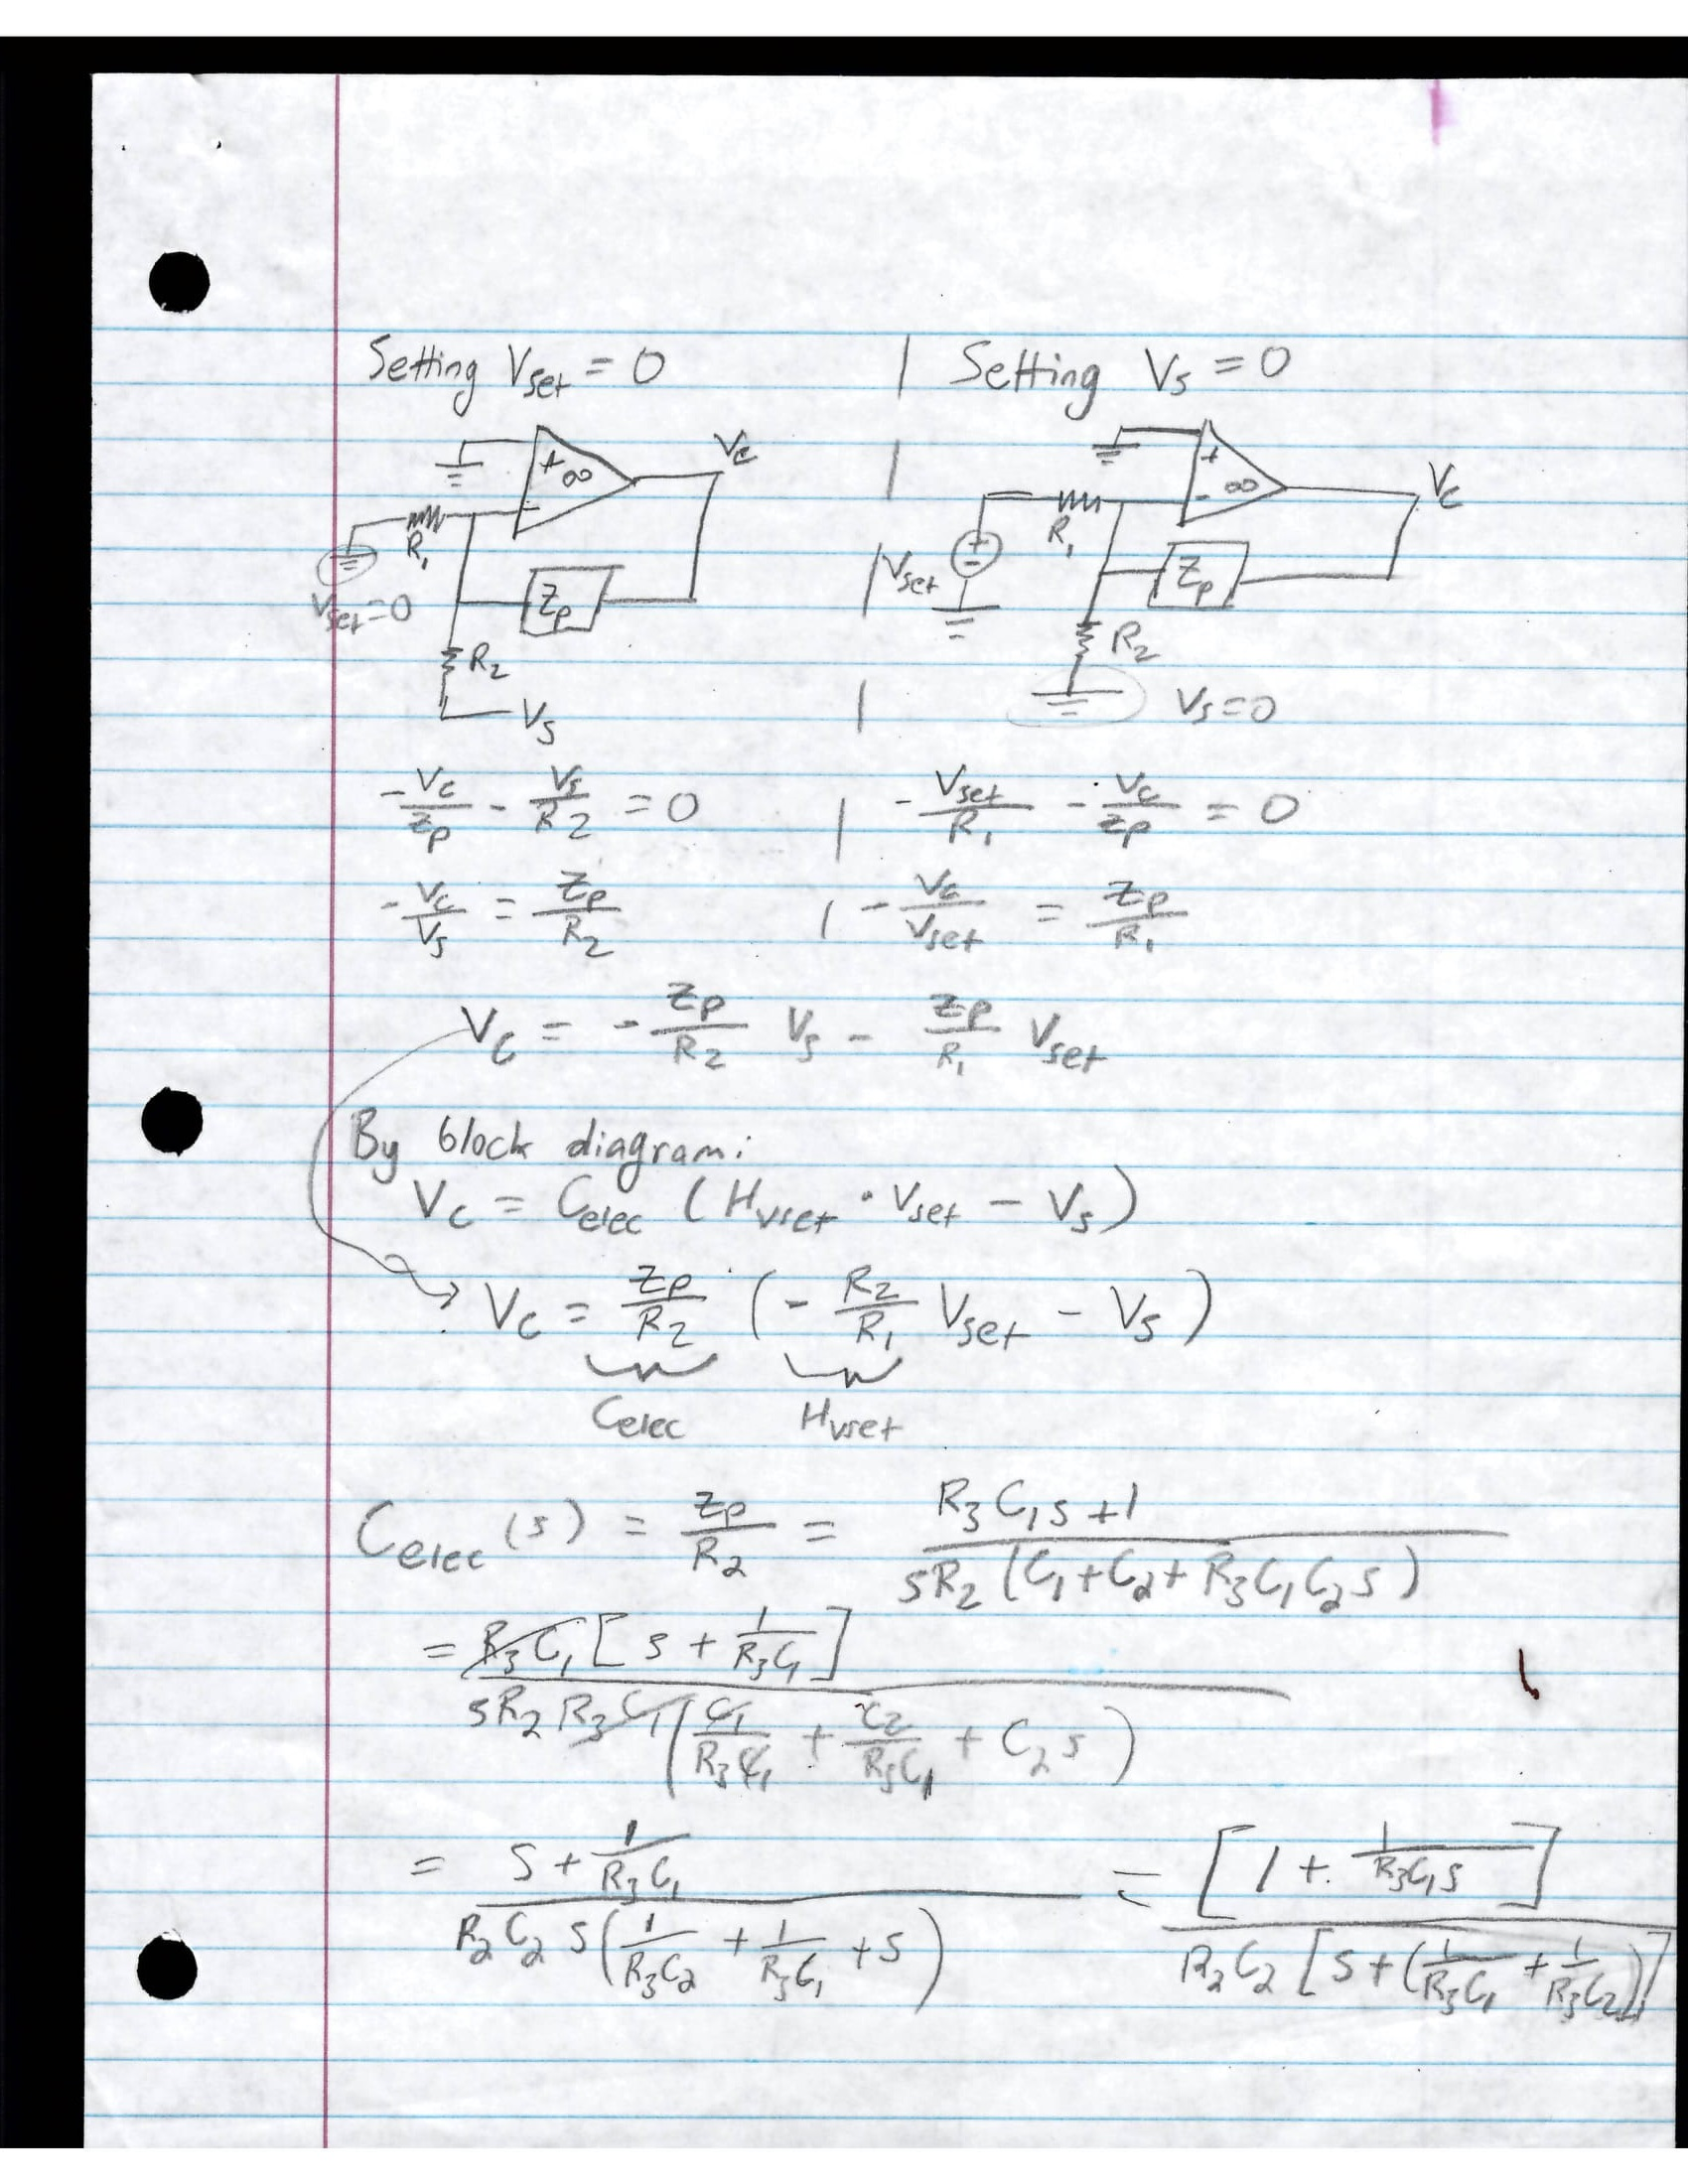
\includegraphics[width=\linewidth]{images/c_elec_2.jpg}
			\end{figure}
			\begin{figure}[H]
				\centering
				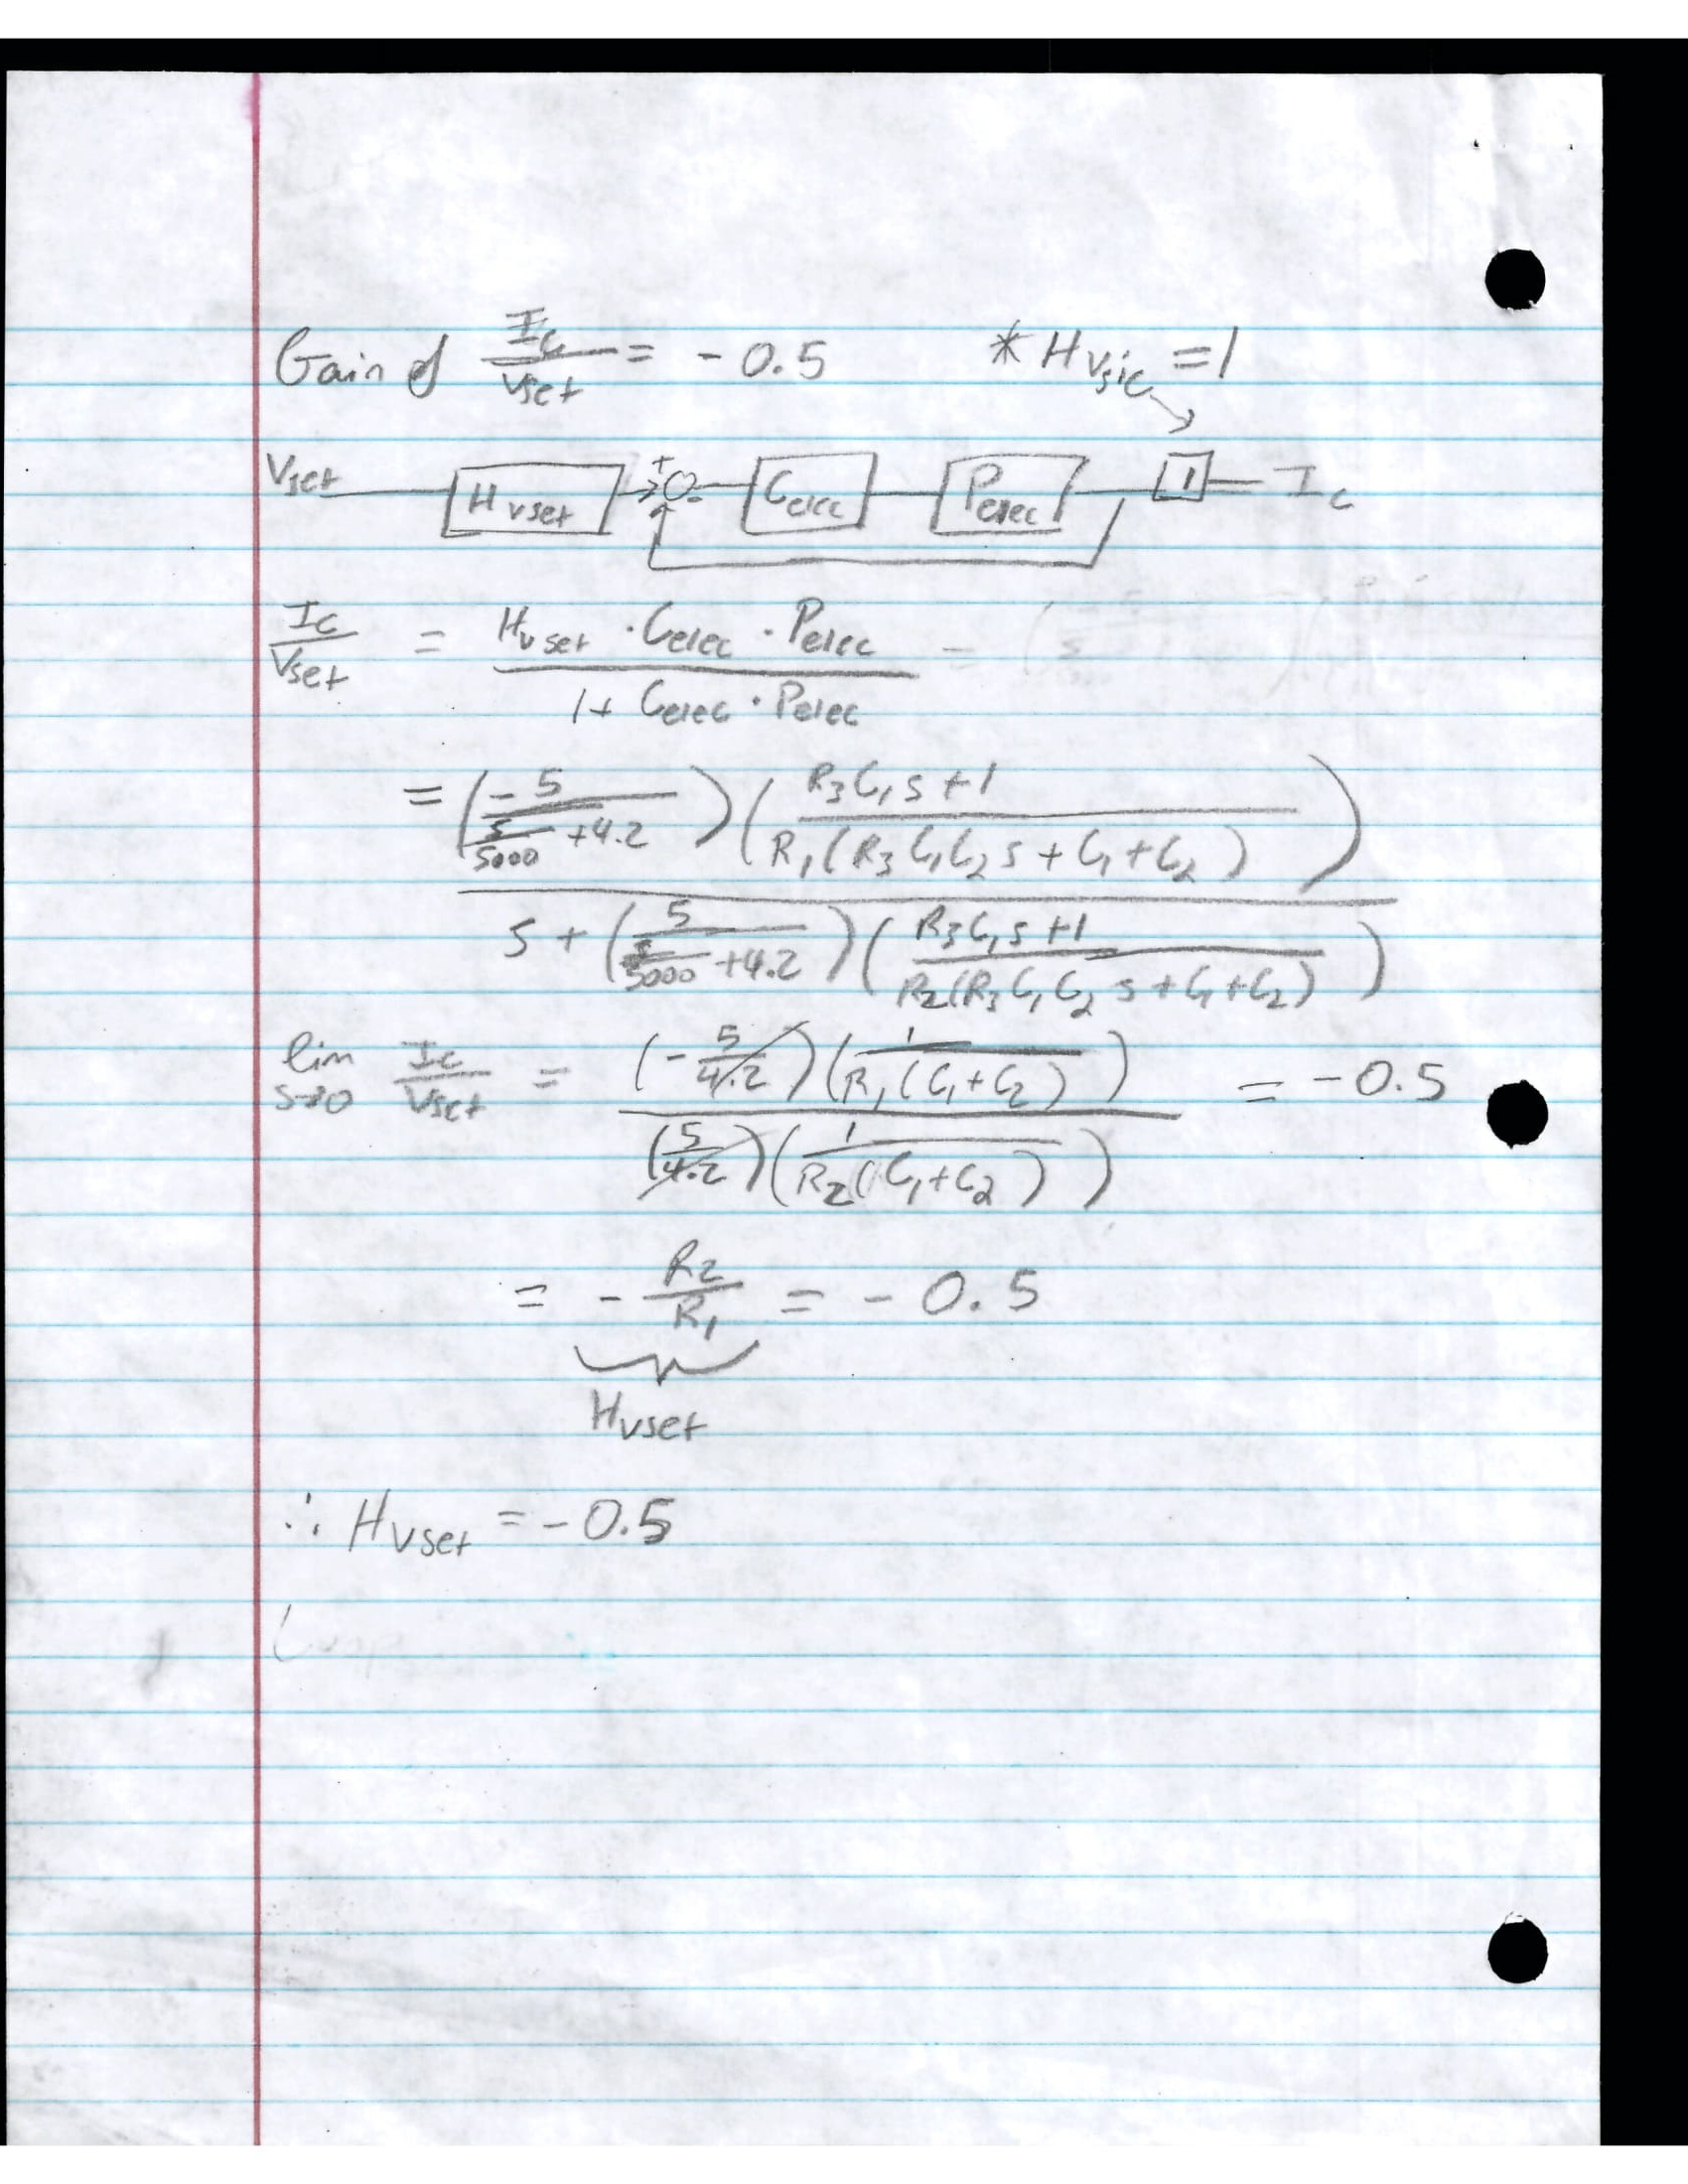
\includegraphics[width=\linewidth]{images/c_elec_3.jpg}
			\end{figure}
			\begin{figure}[H]
				\centering
				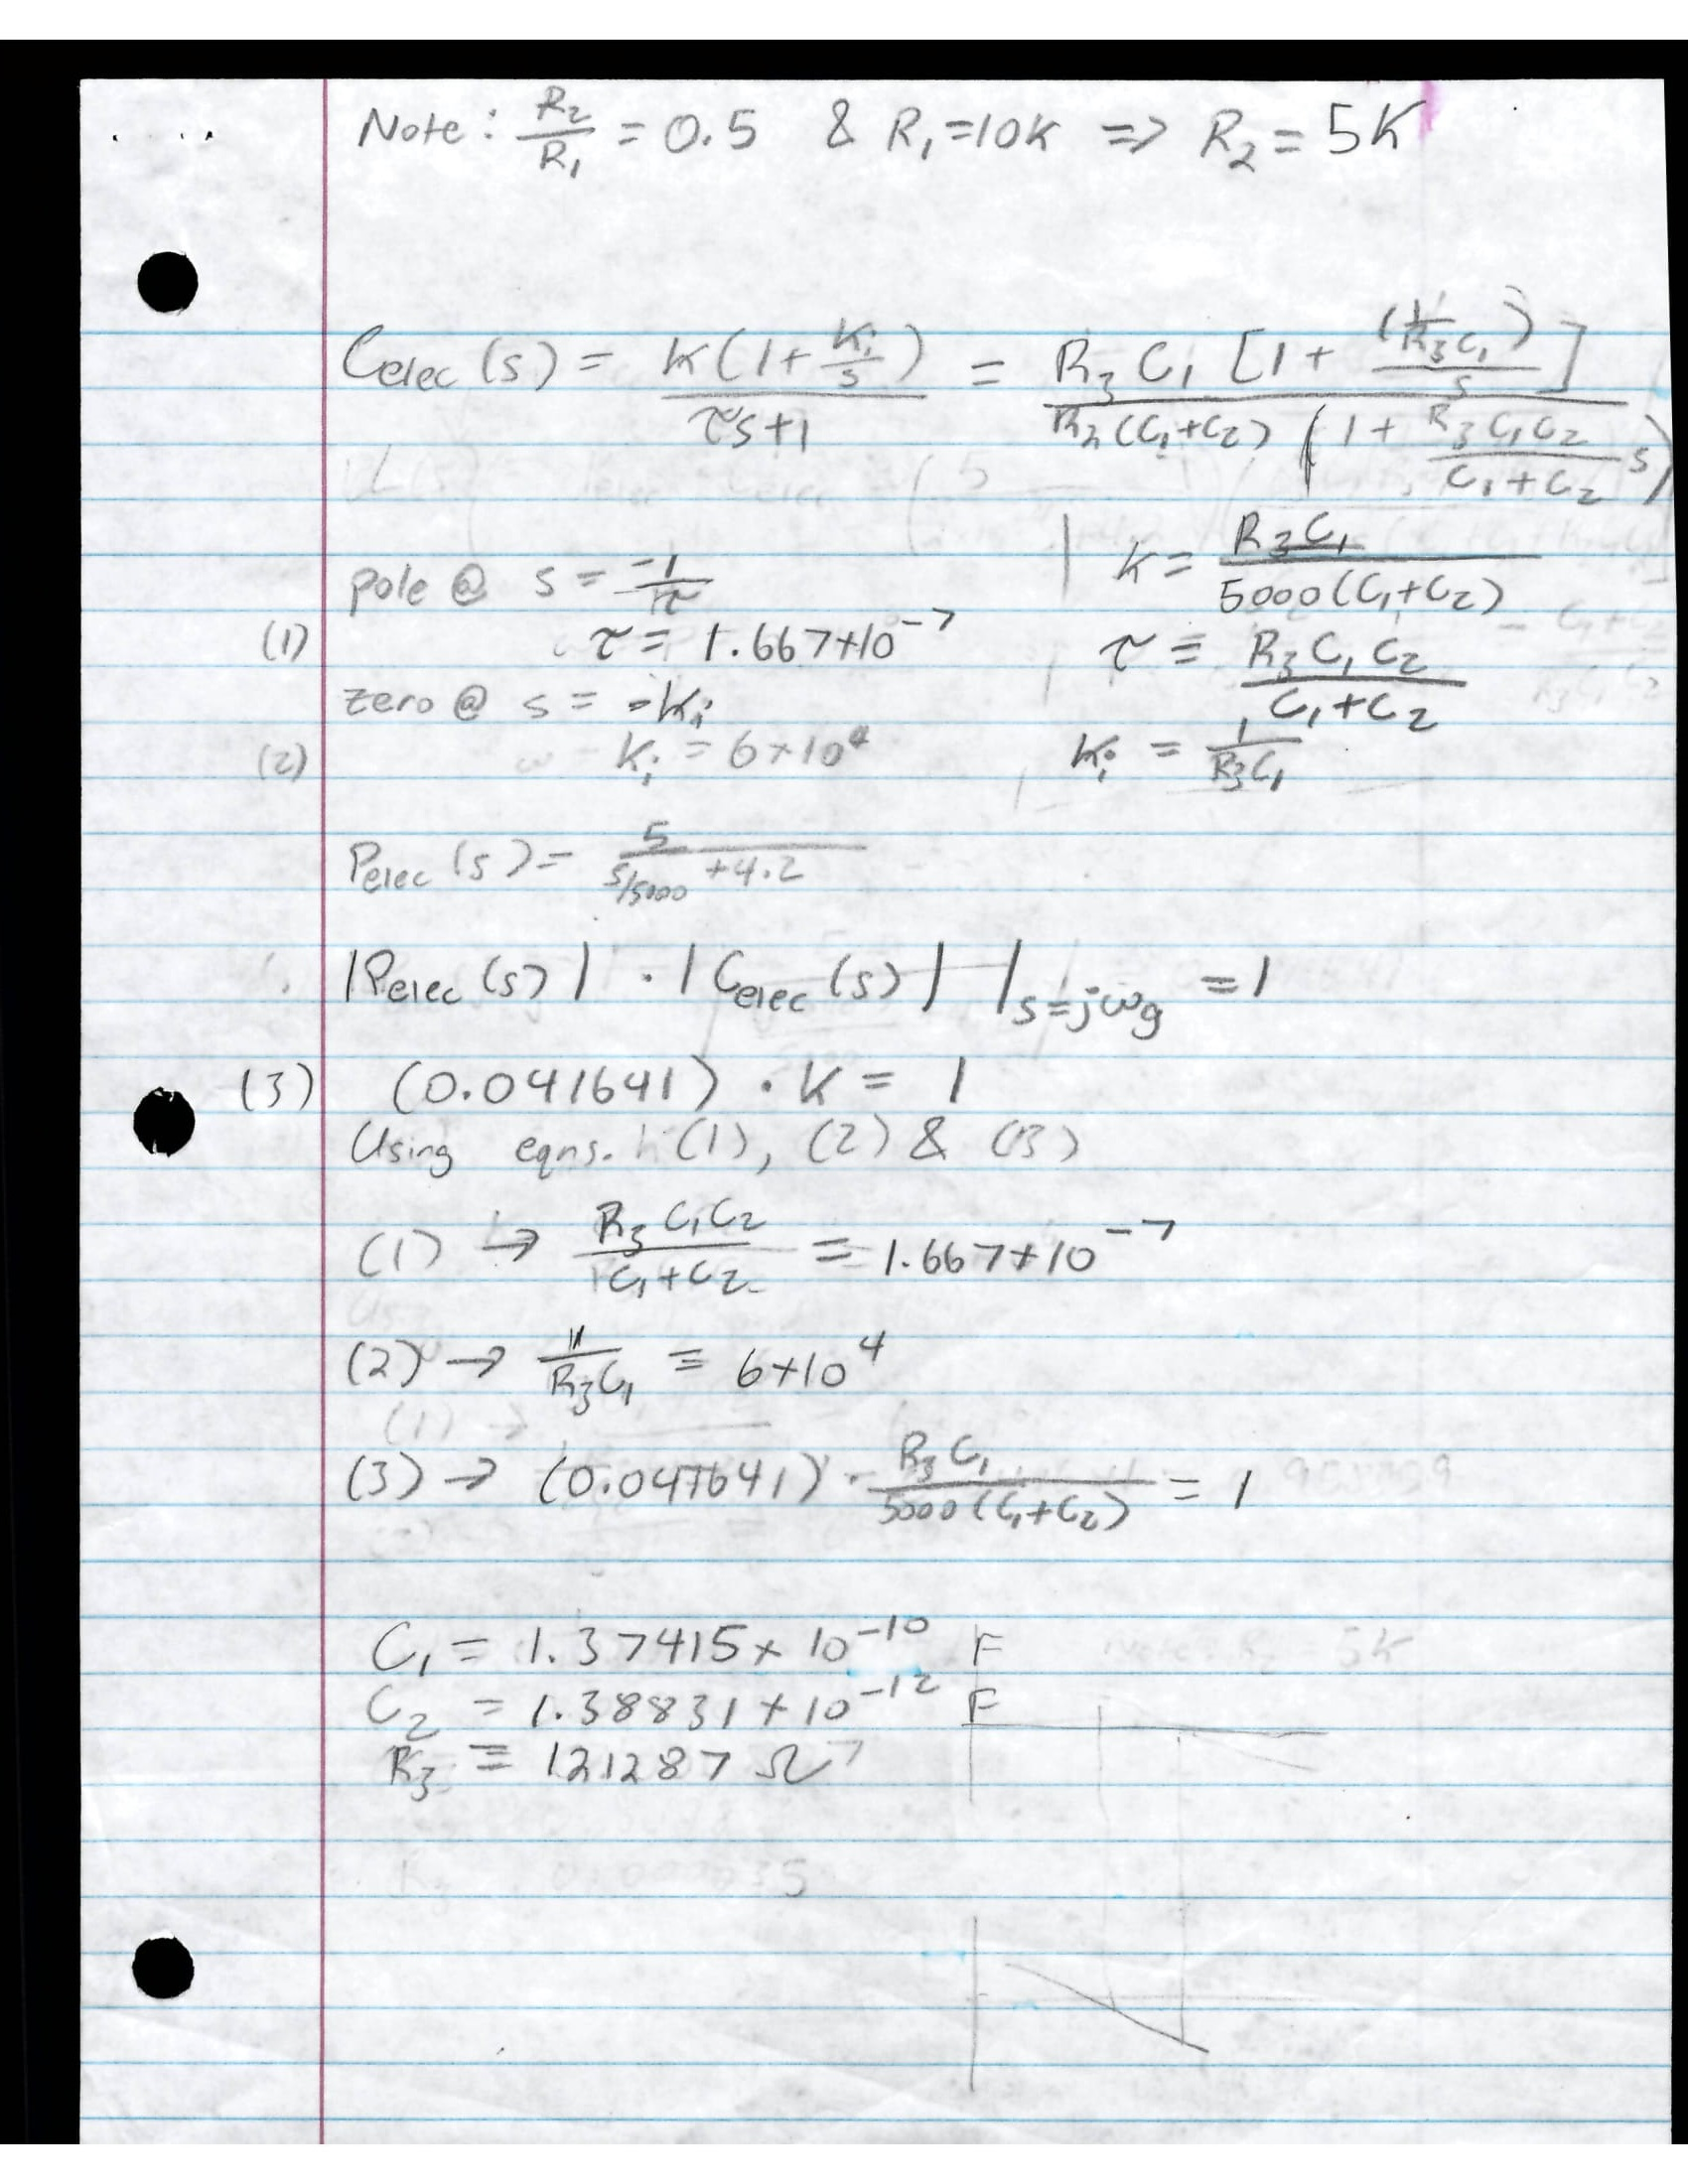
\includegraphics[width=\linewidth]{images/c_elec_4.jpg}
			\end{figure}
			\item Bode plot of Current Loop Transfer Function \\
				The bode plot in the attached Matlab results shows the current
				loop transfer function with the gain crossover frequency
				at $\omega_c = 6*10^5 rad/sec$ and a phase margin of 80.6 degrees.
		\end{enumerate}
		
	\section{FTS Plant System Identification}
		\begin{figure}
			\centering
			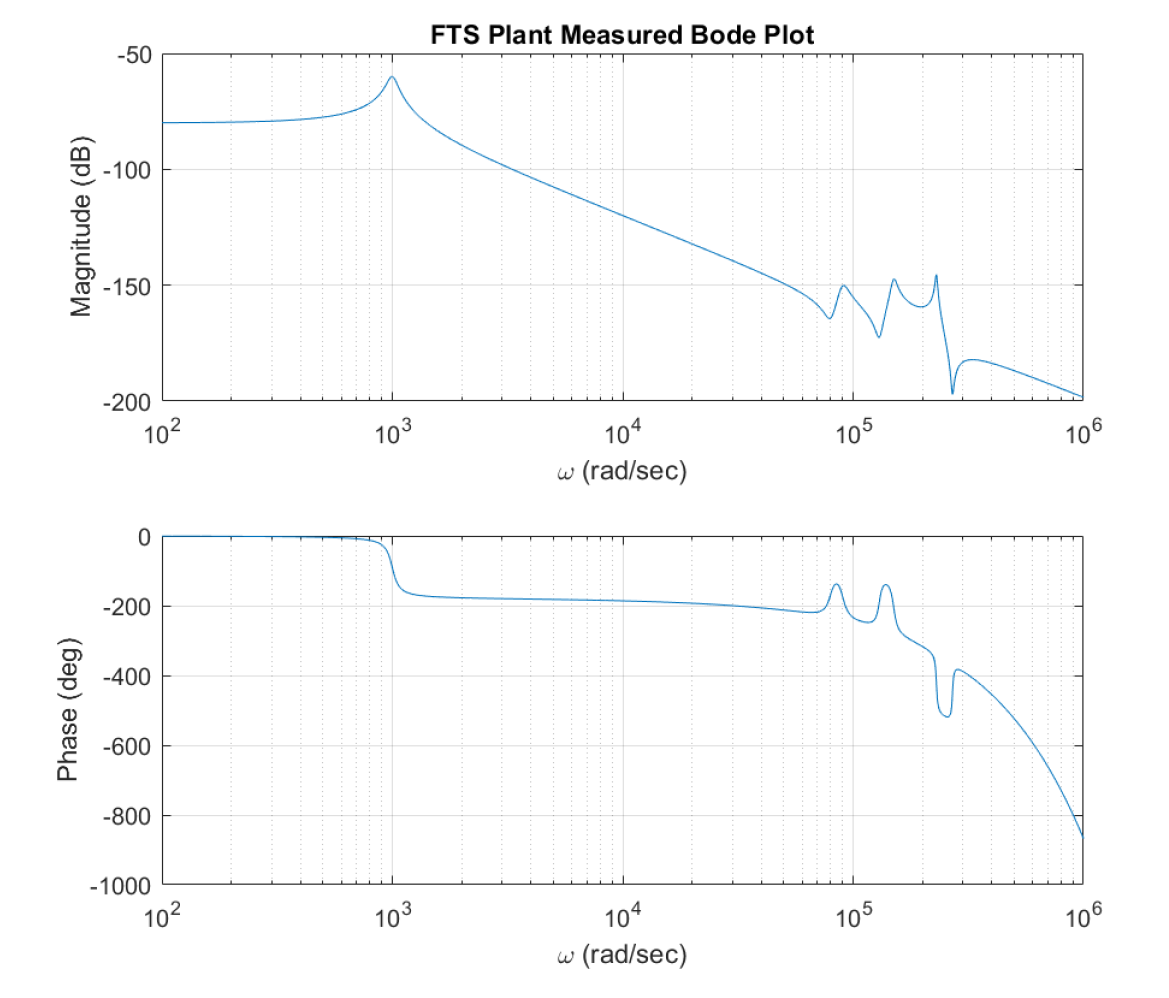
\includegraphics[width=\linewidth]{images/fts_measured_bode.PNG}
			\caption{FTS Measured Data Bode Plots}
			\label{fts_measured_bode}
		\end{figure}
		The measured Bode plot for $G_p(s)$ is given in Figure \ref{fts_measured_bode}.
		In this portion, we used the measured frequency response data to generate a
		transfer function that models the Bode dynamics as shown in Figure \ref{fts_measured_bode}.
		As can be seen in this frequency response data, the mass/spring/damper model
		only accounts for the lowest frequency mode seen on the plot and this lowest mode
		is what we will focus on. In order to arrive at a transfer function that models
		the provided frequency data, we completed the following steps:
		\begin{enumerate}
			\item Find the values for the mass $m_1$, spring constant $k_1$, and the
			damper constant $b_1$ in the simplified FTS model given in Figure \ref{fts_schematics}. \\
			The solutions for these values are given in the derivation below.
			\begin{figure}[H]
				\centering
				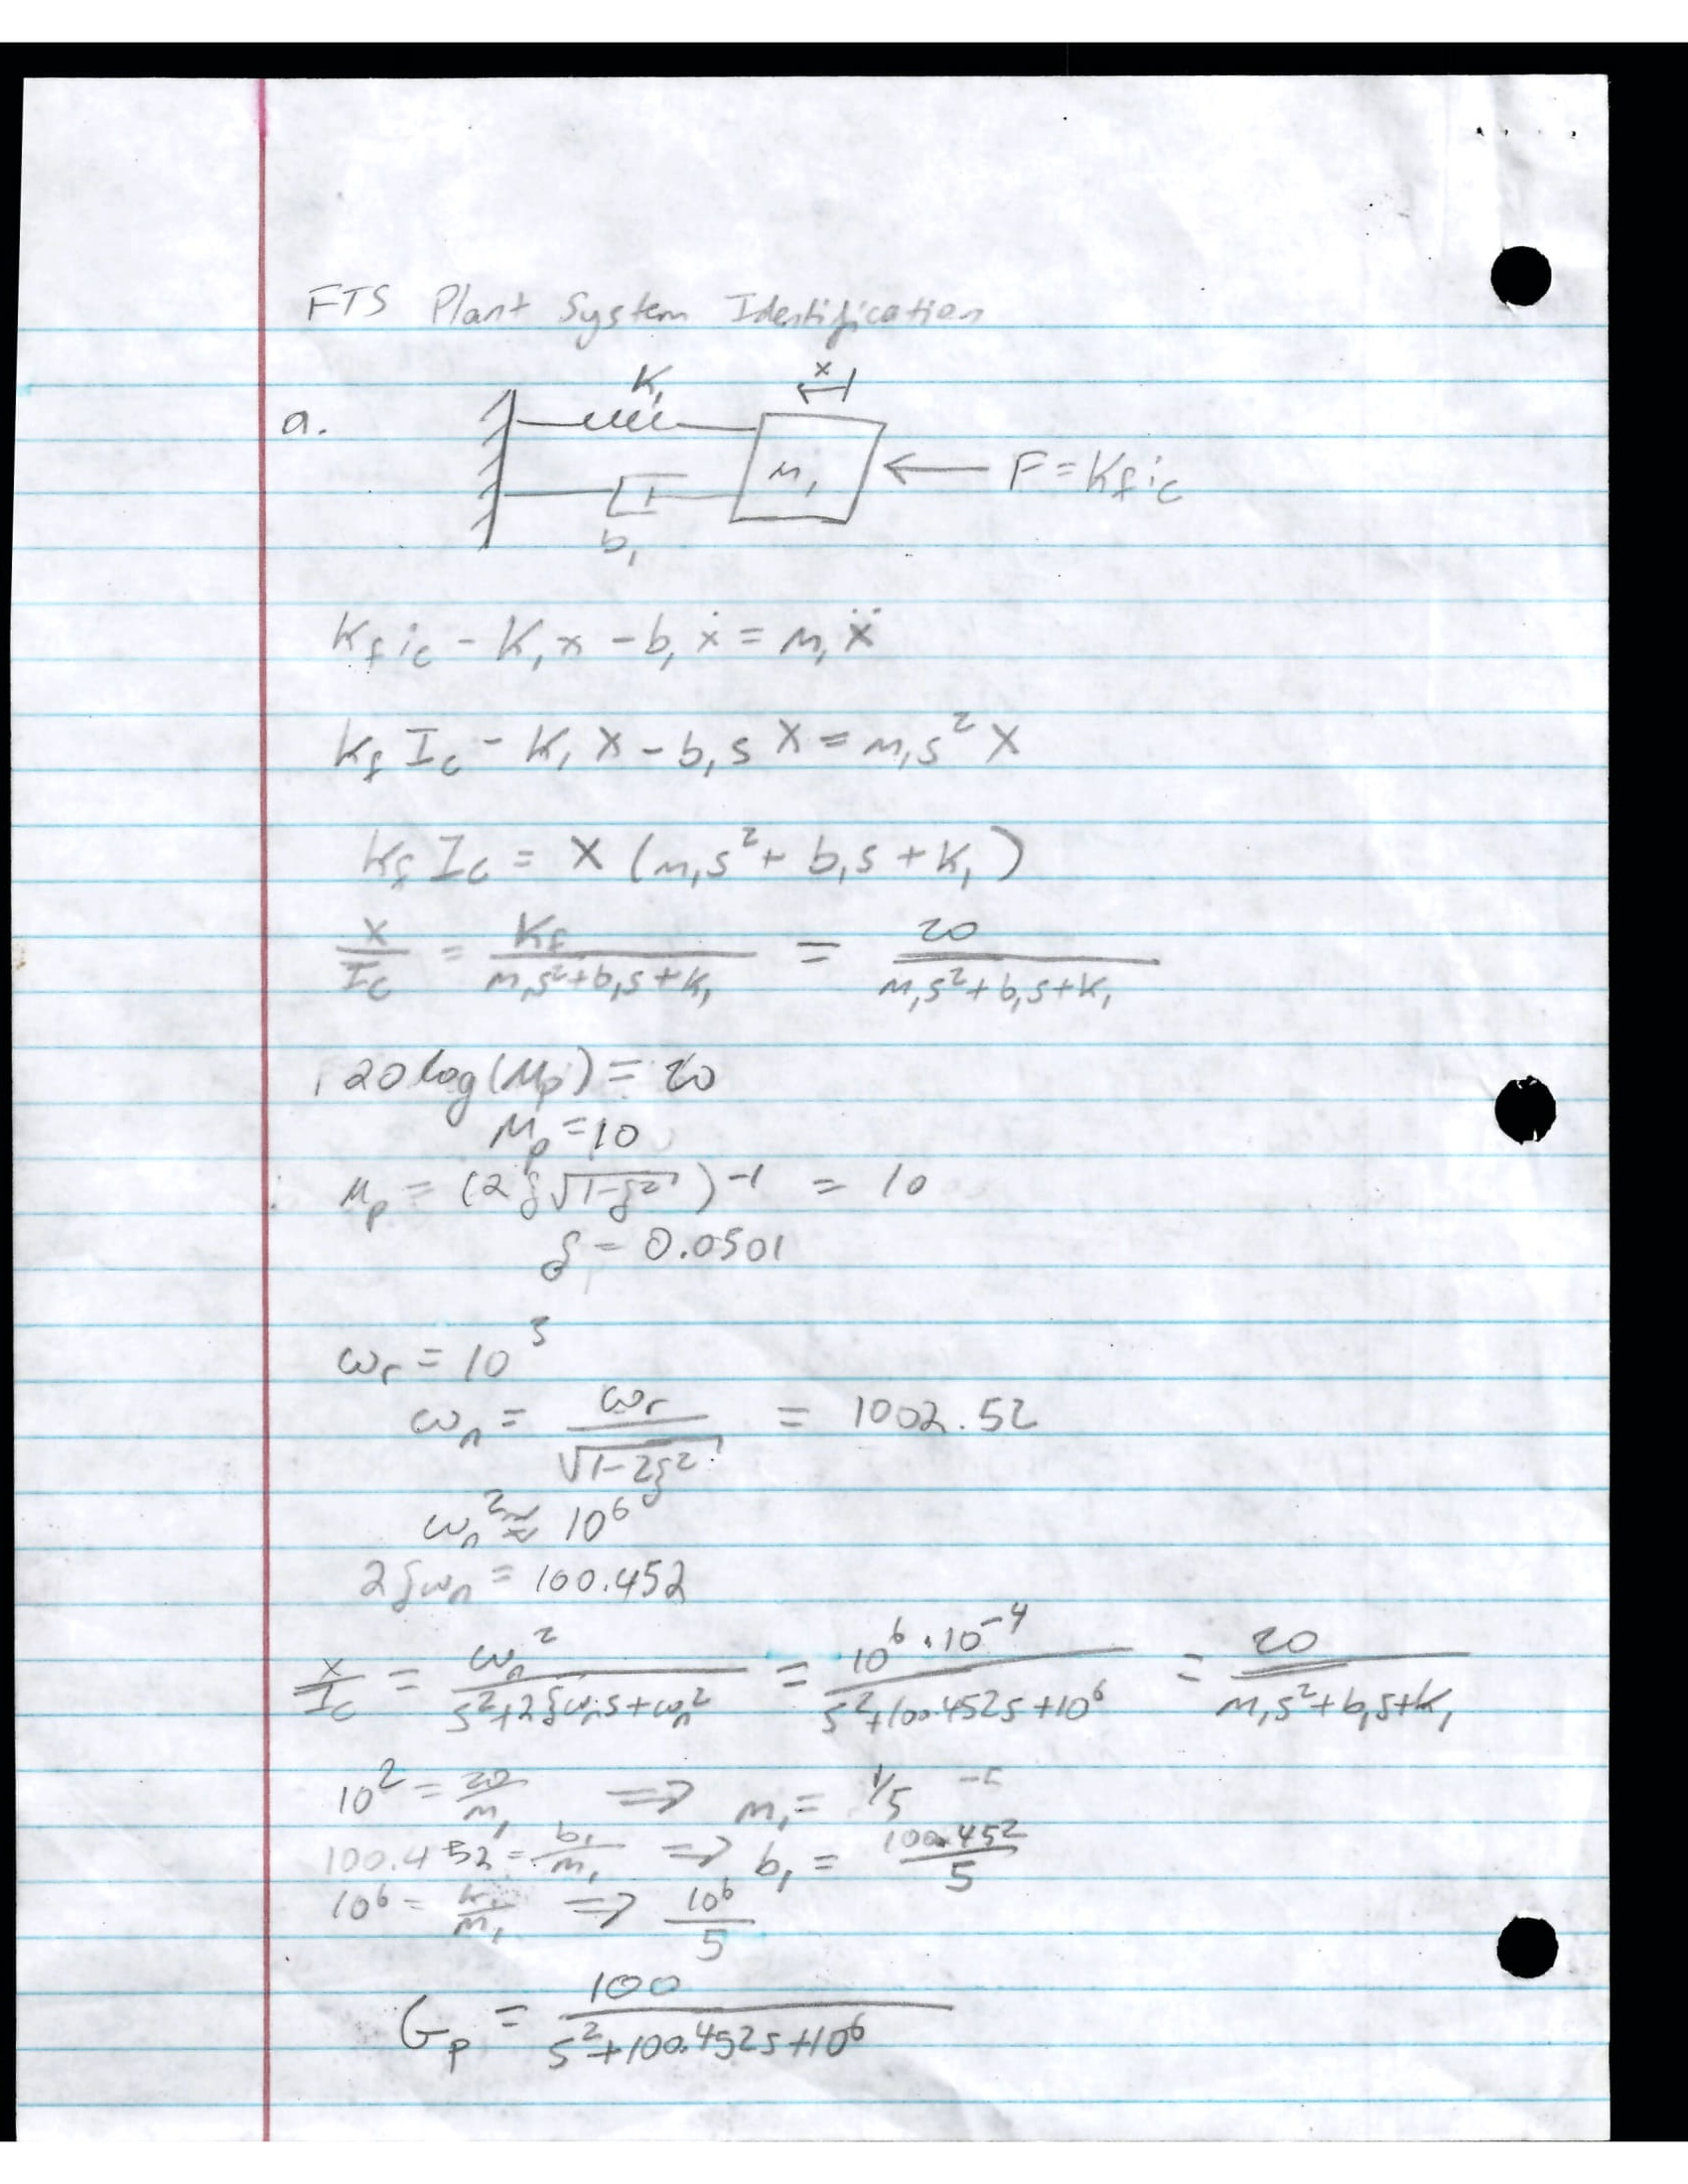
\includegraphics[width=\linewidth]{images/mechanical_derivation.jpg}
			\end{figure}
			\item Fit a dynamical model to the measured Bode plot. \\
			Using the formulas and derivations below, we were able to calculate a model
			for $G_p(s)$ along with an input time delay. We verified this result using
			the frd and tfest commands in Matlab as can be seen by the supplied code.
			\item As can be seen in the Matlab results attached, the bode plots only match
			for the lower frequency mode.
		\end{enumerate}
	\section{Position Control Loop Design}
		The entire position control loop is given in Figure \ref{overall_control_loop}.
		Here, we designed a position controller $C_{mech}(s)$ which gets the error
		between the reference voltage $v_{ref}$ and the sensor output voltage $v_{sense}$
		and generates the voltage $v_{set}$ for the current control loop. Using
		the plant function $G_p(s)$ derived earlier along with the fact that the
		current control loop can be replaced by a constant gain of $G_a = -0.5 A/V$,
		we can create $C_{mech}(s)$.\\
		The controller will have two reference inputs as follows:
		\begin{enumerate}
			\item $1\mu*m$ Constant Position Trajectory: $x_{ref_1}(t) = 10^{-6}u(t) [m]$
			\item Sinusoidal Position Trajectory: $x_{ref_2}(t) = 10^{-5}sin(3000t) [m]$
		\end{enumerate}
		Additionally, the sensor measurement noise can be modeled as:
		\begin{equation*}
			v_n(t) = 5*10^{-2}sin(10^5t)
		\end{equation*}
		The specifications that $C_{mech}(s)$ must adhere to are as follows:
		\begin{itemize}
			\item The closed-loop FTS system is obviously stable
			\item The steady-state position tracking error for the step input is
			almost fully eliminated
			\item The steady-state position tracking error for the sinusoidal input
			trajectory is minimized
			\item The steady-state effect of the measurement noise on the output 
			position is minimized
			\item The magnitude of the closed-loop Sensitivity Function stays below
			+10dB at all frequencies
		\end{itemize}
		Using these criteria, we designed $C_{mech}(s)$ using a PI-lead compensator,
		which takes the form of: \\
		\begin{equation*}
			C_{mech}(s) = K*(1 + \frac{K_i}{s})*(\frac{1 + \alpha\tau*s}{1 + \tau*s})
		\end{equation*}
		Because the noise was at a frequency of $10^5$rad/s and the sinusoidal
		input was at a frequency of 3000rad/s, we decided to shape our loop transfer
		function to increase the gain at high frequency, which results in better
		reference tracking, and reduce the gain at low frequencies, which reduces
		the effect of noise. \\
		To do this, we decided to set our crossover frequency, $\omega_c$ at $10^4$rad/s.
		Also, we wanted to add a phase of roughly $55\circ$ at that crossover frequency
		in order to increase stability and decrease the overshoot as much as possible,
		so we defined our $\alpha$ and $\tau$ using the following formulas: \\
		\begin{equation*}
			\alpha = \frac{1 + sin(\phi_{max})}{1 - sin(\phi_{max})}
		\end{equation*}
		where $\phi_{max}$ is $55\circ$ and
		\begin{equation*}
			\tau = \frac{1}{\omega_c\sqrt{\alpha}}
		\end{equation*}
		Using these equations, we were able to get the form of our lead compensator.
		In order to find the gain values required for the PI portion of the compensator,
		we assumed $K_i$ to be roughly $\frac{\omega_c}{5}$ and let K be a small
		negative number so as to allow the closed loop system to be stable. Then,
		we plotted our system in Matlab and manipulated the gain values until we
		obtained sufficiently small tracking error and a maximum sensitivity level
		under 10dB. \\
		The final compensator was found to be: \\
		\begin{equation*}
			C_{mech}(s) = -0.1(1 + \frac{\frac{3.38*10^4}{5}}{s})(\frac{1+3.1715*10^4*s}{1+3.1529*10^5*s})
		\end{equation*}
		These design choices gave us a strong negative sloped loop transfer
		function passing through the crossover frequency $1.58*10^4$ rad/s. \\\\
		While making these choices we had to take into account the trade off
		between our closed loop transfer T(s) and sensitivity function S(s).
		We learned that T(s)+S(s)=1. This tells us that both T(s) and S(s)
		cannot be minimized, even though ideally that is what we hope to achieve. 
		We saw this manifest itself while we attempted to accomplish the
		specification when the moment we achieved excellent results in the
		closed loop, the sensitivity of our system would go up substantially.
		
\end{document}

